\documentclass[12pt]{article}		
%========================================================
\usepackage{setspace} 	
\usepackage{graphicx}
\usepackage[margin=1in]{geometry}      
\usepackage{hyperref}
\usepackage{xcolor}
\hypersetup{
   colorlinks,
   linkcolor={red!50!black},
   citecolor={blue!50!black},
   urlcolor={blue!80!black}
}		
\usepackage{natbib} 	
\usepackage{float}			
\usepackage{amsmath}	
\usepackage{amssymb}	 			
\usepackage{bm}						
\usepackage{booktabs}
\usepackage{dcolumn}
\usepackage{pdflscape}
\usepackage{afterpage}
\usepackage[hang,flushmargin]{footmisc} 
\setlength\parindent{0pt}	
%========================================================
\newcommand{\X}{\mathbf{X}}
\newcommand{\x}{\mathbf{x}}
\newcommand{\z}{\mathbf{z}}
\newcommand{\Y}{\mathbf{Y}}
\newcommand{\K}{\mathbf{K}}
\renewcommand{\k}{\mathbf{k}}
\newcommand{\bc}{\mathbf{c}}
\renewcommand{\r}{\right}
\renewcommand{\l}{\left}
\newcommand{\bomega}{\bm{\omega}}
\newcommand{\bpsi}{\bm{\psi}}
\newcommand{\bbeta}{\bm{\beta}}
\newcommand{\balpha}{\bm{\alpha}}
\newcommand{\bphi}{\bm{\phi}}
\newcommand{\btheta}{\bm{\theta}}
\newcommand{\dist}{\buildrel\rm d\over\sim}
\newcommand{\ind}{\stackrel{\rm indep.}{\sim}}
\newcommand{\ud}{\mathrm{d}}
\newcommand{\iid}{\stackrel{\rm i.i.d.}{\sim}}
\newcommand{\logit}{{\rm logit}}
\newcommand{\cA}{\mathcal{A}}
\newcommand{\E}{\mathbb{E}}
\newcommand{\V}{\mathbb{V}}
\newcommand{\cJ}{\mathcal{J}}
\newcommand{\bone}{\mathbf{1}}
\newcommand{\var}{{\rm Var}}
\newcommand{\cov}{{\rm Cov}}
\DeclareMathOperator*{\argmin}{\arg\!\min}
\DeclareMathSizes{10}{12}{10}{10}
%========================================================
\begin{document}

\title{Predicting Foreign Fighter Flows to Syria Using Machine Learning: An Introduction to Kernel Regularized Hurdle Negative Binomial\thanks{The authors are listed in alphabetical order, and contributed equally. We thank Bryce Dietrich, Chad Hazlett, Jeff Lewis, David Rapoport, Art Stein, and Barbara Walter for their feedback. We also benefited from comments at the UCLA Comparative Politics Reading Group, and the 2016 Midwestern Political Science Association Conference. The usual disclaimer applies. For replication material and our companion software---still in its developmental phase in \texttt{R}---see \href{https://github.com/lukesonnet/foreign_fighters}{https://github.com/lukesonnet/foreign\_fighters}.}}

\author{George Derpanopoulos\thanks{PhD Student, Dept. Political Science, UCLA. Email: \href{mailto:gderpa@ucla.edu}{\tt gderpa@ucla.edu}} \and Luke Sonnet\thanks{PhD Student, Dept. Political Science, UCLA. Email: \href{mailto:luke.sonnet@gmail.com}{\tt luke.sonnet@gmail.com}}}

	\maketitle
%=========================================================
	\thispagestyle{empty} 
	\singlespacing

\begin{abstract}	
Why have some countries counted hundreds of their citizens fleeing to fight in Syria, while other countries' citizens have remained bystanders? There are three methodological challenges to answering this question. First, there may be two groups of countries: one at no risk of ``supplying'' foreign fighters and another supplying some positive amount. Second, there is no clear theory to specify the functional forms linking features to foreign fighter supply. Third, existing models perform poorly out of sample or yield output that is not amenable to social-scientific interpretations. To solve these challenges, we augment a hurdle negative binomial model with two machine learning tools. Namely, we allow our features to affect the response non-parametrically by using kernel functions that represent expansions of the data. Furthermore, we add regularization terms that penalize complexity to mitigate overfitting. Our approach combines the strengths of predictive and confirmatory models: it performs similarly to state-of-the-art machine learning algorithms in prediction while providing substantively interpretable output.  Applying our model to data on 163 countries, we find that populous, developed countries, with a large Sunni population and proximity to Syria supply more fighters. These results lend themselves to viewing foreign fighter supply as largely driven by structural forces.
\end{abstract}

%=========================================================
	\newpage
	\setcounter{page}{1} 			
	\onehalfspacing

\section{Introduction}

The ongoing Syrian Civil War has been named ``the world's largest humanitarian crisis since WWII'' \citep[p. 1]{ECHO2015}. 230,000 dead, 850,000 injured, 4 million refugees, and 7.5 million internally displaced; these are some conservative estimates of the conflict's cost.\footnote{All figures are the most recent estimates that could be found as of June 2015 \citep{UNOCHA2015}.} An integral component of the conflict are the multiple rebel groups involved, like Islamic State, Jabhat al-Nusra, and the Free Syrian Army. Although rebel manpower is hard to estimate, there is consensus that a significant portion of it comes from foreign fighters \citep{Byman2015}, ``non-state actors involved in military activity in a foreign country'' \citep[p. 1]{Hegghammer2013}. Moreover, with an estimated 21,000 foreigners from 50 countries fighting in Syria \citep{Neumann2015}, foreign fighter supply has reached a historical high \citep{Hegghammer2013a}. \\

Naturally, policy-makers are asking themselves what draws their voters to participate in a foreign conflict. Common concerns were best expressed by Britain's Prime Minister, David Cameron: ``one of the most disturbing aspects is how this conflict is sucking in our own young people, from modern, prosperous societies''. So far, public discourse has addressed these concerns by focusing on individual fighters' motivations. This has been complemented by an emerging case-study literature based on returning fighter interviews \citep{Stenersen2011, Weggemans2014, Nilsson2015}. As a result, a popular conception of foreign fighters has emerged; that of young Muslims from poor urban environments, with ``deep-seated feelings of marginalization and exclusion'' \citep[p. 2]{Noor2014}.  \\

Whether the inferences of this literature are accurate and generalizable is an open question. Before settling it, though, policy-makers might want to know what the role of \textit{country-level} features is in individual fighters' calculus. In particular, we might ask to what extent can foreign fighter supply be attributed to \textit{policy}, which is under the control of government, versus countries' \textit{structural features}, which are sticky. To date, there is no study addressing these questions. However, the ongoing nature of the conflict, its spillovers into the region, and the continuing flow of fighters throughout the globe call for a systematic analysis of the evidence. We take a first step in that direction, thereby responding to the recommendations of policy reports, that ``strategies would benefit immensely from more evidence-based research'' \citep[p. 17]{GCCS2014}. \\

An analysis of the predictors of foreign fighter supply is hindered by two classes of problems: data availability and modeling challenges. In this study, we focus on overcoming the difficulties in modeling this process. Namely, our approach addresses four sets of issues, relating to our priors about the country-level mechanism generating foreign fighter supply, the nascent state of the literature, and our dual interest in prediction as well as inference and interpretability. \\ 

First, our theory-motivated prior that foreign fighter supply is a two-component process---some function of countries' features should predict \textit{whether} they supply any foreign fighters and, if so, another function should predict \textit{how many} fighters they supply. This is motivated by qualitative evidence that supplying at least one fighter alters supply dynamics within a country; radicalization and recruitment networks form, along with policies to contain them, and a different mechanism takes over the ``scaling-up" of supply. Such a theoretical structure suggests that a two-component mixture model is appropriate, with one component predicting assignment to supplier countries (binary response), and a second component predicting the number of fighters supplied (count response left-truncated at $1$). This directs us to the familiar hurdle model \citep{Mullahy1986}. In addition, the count nature of the response and its large variation urge us to further refine our specification to the hurdle negative binomial model.  \\

As with any mixture model, we can allow different features, or different functions of the same features, to enter each component. However, this brings us to a second modeling challenge: there is little theory on how a country's features combine to affect foreign fighter supply, let alone how this should vary between the model's components. The assumption behind most regression models is that the systematic component of a unit's response is a linear function of its features \citep{King1989a}. When models are specified using vague theoretical priors, though, parametric assumptions are hard to justify \citep{Ho2007}. Instead, model-fitting could greatly benefit from a flexible semi-parametric approach. Semi-parametric and non-parametric models are not uncommon, yet existing models do not allow us to impose the theoretically-motivated structure of the hurdle model. \\

Another downside of many non-/semi-parametric models is that they overfit the data, thereby yielding poor out-of-sample predictions -- a third challenge to address. This can be addressed by machine learning algorithms that penalize complexity, like LASSO and Random Forest. Regularizations based methods like the LASSO or Ridge regression use $k$-fold cross-validation to tune penalty, or regularization parameters in order to strike a better balance on the bias-variance tradeoff than classical estimators. Unfortunately, though, semi-parametric regularized models give way to a fourth challenge: they do not produce quantities of interest familiar to social scientists, like marginal effects and confidence intervals. In fact, demanding such quantities of interest requires sacrificing flexible model-fitting---for example, output from ridge regression is interpreted like that of GLMs, but the model assumes that the features affect the response linearly.  \\

In short, we seek an algorithm that combines attractive features from multiple approaches: the intuitive structure of the hurdle model, the agnosticism of non-parametric models on how the features combine to affect the response, the good out-of-sample performance of regularized algorithms, and the interpretability of standard regression models. We bridge the generalized linear model and machine learning literatures to arrive at such an algorithm, the Kernel Regularized Hurdle Negative Binomial (KRHNB). Specifically, we derive our estimator by applying kernel expansion and regularization to a hurdle negative binomial, then develop companion software to compute parameter estimates that minimize prediction error, produce pointwise marginal effects, and get bootstrapped estimates of uncertainty. \\

Our procedure consists of several simple steps. We begin by assuming the data is generated by a two-component mixture model: a logit predicting whether a positive count is observed and a negative binomial (left-truncated at $1$) predicting the conditional count. Then we form the sample log-likelihood function and add a regularization term (using an $L_2$ norm), thereby arriving at our target function---the penalized log-likelihood. To move away from a fully parametric form, we expand our feature matrix into a higher-dimensional space; in our application we use an infinite-dimensional space corresponding to all possible expansions of the data (e.g. polynomial, logarithmic, exponential, multiplicative). This makes our target function linear in the \textit{mapping} of the features, instead of the features themselves. We then show that the features enter the minimum of the target function solely through inner products and thus can be substituted by positive semi-definite kernels, like the Gaussian kernel. This is known as Mercer's Theorem and enables numerical optimization of the target function. \\

Predicted responses are derived by substituting our estimates into the hurdle negative binomial's conditional expectation function (CEF). Pointwise marginal effects for feature $j$ are computed using numerical derivation of the CEF with respect to feature $j$. Averaging these effects for each feature gives us its average pointwise marginal effect. Finally, redrawing $1,000$ samples from our data with replacement and repeating the above computations gives us non-parametric bootstrapped estimates of uncertainty---a distribution of average pointwise marginal effects for each feature. All relevant computations are performed with our companion software, written in the \texttt{R} language.	\\

KRHNB has two attractive properties over the standard hurdle negative binomial. First, regularization penalizes complexity, thereby striking a better balance on the bias-variance tradeoff. Thus, our procedure is less prone to overfitting the training data and better predicts test data. Second, feature expansion implicitly allows our features to affect the systematic component of the response through any functional form. This is particularly valuable in this context; the absence of theories of country-level foreign fighter supply should deter us from making strong parametric assumptions. Nevertheless, one might ask: does our method improve over other machine learning models? After all, there are other algorithms that penalize complexity, some of which impose less structure on the data.   \\

To answer this question, we compare our method to three popular machine learning algorithms and find that it performs better or comparably to all of them. Using a cross-section of 163 countries, and an array of 27 demographic, economic, geographic, and political features, we compute the leave-one-out cross-validation root mean square error and the mean absolute error. Higher mean absolute error rates are produced by all 3 of our benchmark models: Kernel Regularized Least Squares (KRLS) \citep{Hainmueller2013}, KRLS truncated at 0, and a Random Forest. Only Random Forest outperforms KRHNB with respect to root mean squared error and this is largely due to its relative success in predicting a few large outliers. \\

Having established the merits of our approach -- theoretical motivation, flexibility, predictive power, and interpretability -- we apply it to our data, in an effort to contribute to the literature on foreign fighters. Substantively, we find that structural features dominate in predicting foreign fighter supply: populous, developed countries, that are close to Syria, and have a high concentration of Sunnis supply more fighters. Some features that respond to government policy more easily also matter: internet usage, refugee intake, government regulation of religion, and government favoritism of a particular religion positively predict foreign fighter supply. Our method also lends itself to the discovery of interesting heterogeneity in the predictive effect of our features. We find that the positive relationships of refugee intake and government regulation of religion with foreign fighter supply stem from European and Muslim-majority countries, respectively. Throughout this paper, we refer to effects in the sense of partial derivatives; we do not make causal claims.	\\

To the limited extent that our research design allows us to inform policy, the implications of our findings for constraining foreign fighter flows are grim: little can be done and what can be done is costly. This is because the strongest and most accurate predictors of foreign fighter supply are structural features, while the cost of altering policies that predict supply might exceed the benefit of curbing it; in European countries, reducing refugee intake would arguably alienate the median voter, while in Muslim-majority countries, liberal government policies towards religion might be resisted. Furthermore, the relationships uncovered by this analysis say little about the general equilibrium effects of a large shift in government policy.    \\

The remainder of this study proceeds as follows. Section \ref{sec:background} provides background information on the Syrian Civil War and foreign fighters. Section \ref{sec:theory} reviews the emerging literature on foreign fighter supply and synthesizes a theoretical framework to analyze the data. Section \ref{sec:hurdles} outlines some obstacles to empirical modeling in this setting, and motivates our method. Section \ref{sec:krhnb} presents the theory and mechanics of KRHNB. Section \ref{sec:computation} covers issues related to modeling choices and computation. Section \ref{sec:comparison} compares our predictions to those of other models. Section \ref{sec:results} displays the substantive findings of our analysis and provides possible substantive interpretations. Finally, Section \ref{sec:conclusion} summarizes, underlines the limitations of our approach, and suggests directions for future research. 

%=========================================================
\section{Foreign Fighters in Syria}	\label{sec:background}

Foreign fighters are not a novel fighting technology. They have existed since at least the Greek War of Independence in the 1820s, have participated in different types of conflicts (ethnic, political, religious), and in several regions of the world (Europe, Asia, Latin America, Africa) \citep{Malet2010}. However, the scale of foreign fighter presence in Syria is unprecedented. Conservative estimates place it around $21,000$, far exceeding supply to conflicts in the past 40 years, like those of Afghanistan, Bosnia, or Somalia \citep{Hegghammer2011}. Already, confirmed cases of foreign fighters have been noted in $50$ countries \citep{Neumann2015} -- their supply is mapped in Figure \ref{fig:ff_map}. \\

\begin{figure}
	\centering
	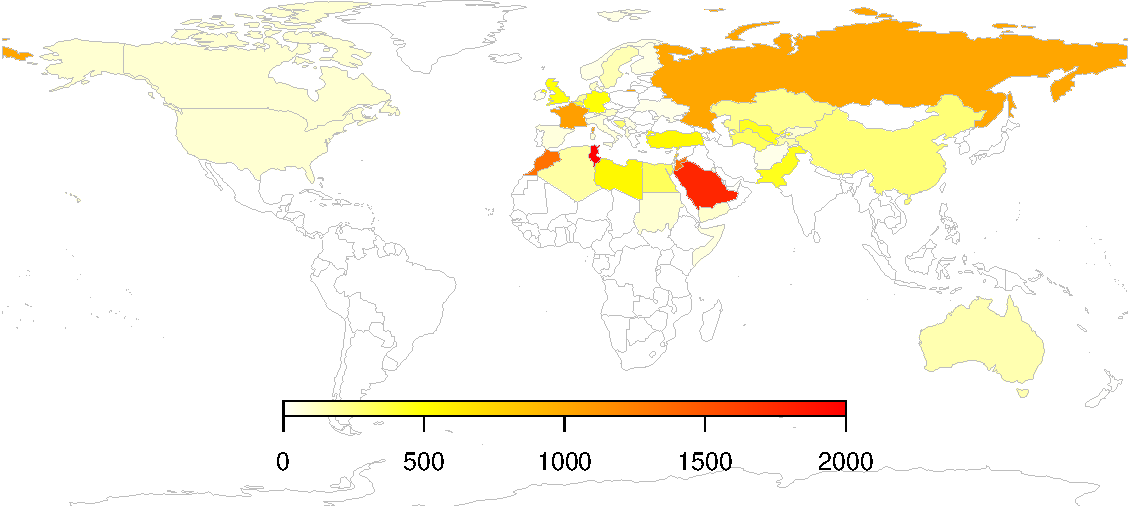
\includegraphics[width = \linewidth]{tabs_figs/worldMap_edited.pdf}
	\caption{Global Distribution of Foreign Fighter Supply, Through 2014 \citep{Neumann2015}}	\label{fig:ff_map} 
\end{figure}

The scale of the foreign fighter phenomenon has raised a number of concerns in both Syria and supplier countries. Regarding the conflict itself, there is concern that foreign fighters may swing outcomes. Indeed, there is anecdotal evidence that insurgencies with foreign fighters are more successful \citep{Hegghammer2011, Malet2010}. Moreover, the Syrian case is complicated by the presence of multiple organizations with competing ideologies. On the one hand, groups like the Free Syrian Army (FSA) promise a secular, democratic and pro-Western government upon toppling Assad. On the contrary, groups like Islamic State (IS) strive to replace the Ba'athist regime with an Islamic caliphate. To the extent that both of these opposing camps are continuously strengthened by foreign fighters, it is unlikely that either will prevail. Hence, even if insurgents succeed in defeating the state, factional conflict will make a ceasefire unlikely.\footnote{The dynamics are complicated further if we consider Hezbollah and other Shia or pro-government militias' support of Assad.} 	\\

Just as many concerns have been raised in the countries where foreign fighters originate. Despite some governments taking an active stance on the conflict, they do not condone their citizens' participation, even if it is in support of an organization allied with their government (e.g. FSA).\footnote{In order to deter their citizens from joining the conflict, some governments have passed legislation to revoke returning fighters' citizenship (e.g. Australia, Britain, Canada, USA). See \href{http://news.nationalpost.com/news/canada/canadian-government-revoking-passports-of-citizens-trying-to-join-extremist-groups}{http://news.nationalpost.com/news/canada/canadian-government-revoking-passports-of-citizens-trying-to-join-extremist-groups}.} More problematic is the case of foreign jihadis, since a coalition of numerous countries has declared war on groups like IS, yet some jihadis are citizens of these countries. A prominent example is ``Jihadi John'', a British citizen---and IS fighter---that was bombed by air strikes funded through his taxes. Cases like this have troubled Western governments, whose citizens comprise an estimated $20\%$ of foreign fighters in the conflict.\footnote{This estimate is based on the data we employ \citep{Neumann2015}. In this case, the West is defined as non-Muslim-majority countries.} \\

In addition to shaking the liberal-democratic foundations of these countries, the greatest concern relates to the ``veteran effect'': the risk of returning fighters carrying-out terror attacks in their home country \citep{Hegghammer2013}. Veterans' training, experience in combat and access to networks of fighters makes them prime candidates for terrorist recruiting, with \cite{Hegghammer2011} claiming that ``most transnational jihadi groups today are by-products of foreign fighter mobilizations'' (p. 53). Naturally, policy-makers are worried that their citizens can participate in foreign conflicts and then import violence to their home country.	\\

A similar pattern holds in the literature. Few studies ask what causes one to become a foreign fighter, while virtually none focuses on country-level features. Crucially, ignoring these features impedes our ability to prevent foreign fighter flows in future conflicts. Admittedly, the Syrian conflict is well underway, and thus the most efficient way to minimize its costs is to contain its spillovers. In future cases, though, given that prevention is cheaper than treatment, a more efficient strategy is to identify potential supplier countries. This will also benefit countries on the receiving end; negotiation is always preferable to conflict, but the potential inflow of fighters makes conflict more likely.   \\

This study takes the first step towards predicting country-level foreign fighter flows. Before proceeding, though, in the next section we briefly review the emerging literature on foreign fighters and synthesize it into a broad theoretical framework. We do not put forth an argument for how foreign fighter flows take shape at the country level, let alone the individual level. We simply impose the minimum theoretical structure necessary to later enable a substantive interpretation of our findings. 

%=========================================================
\section{Predictors of Foreign Fighter Supply}	\label{sec:theory}

The literature on foreign fighters is still in its nascent stage, yet combines insights from a range of disciplines: political science, history, sociology, public policy, security, and counter-terrorism studies. A comprehensive review of this work is beyond our scope, and instead we focus on studies that touch on the determinants of foreign fighter supply. Unfortunately, we are aware of only one study that explores \textit{country}-level predictors \citep{Hewitt2009}; remaining studies and policy reports tackle the question at the individual level.	\\ 

Crucially, although we extract the covariates that feature in this literature to synthesize a framework for country-level explanations of foreign fighter supply, we do not claim to \textit{test} the theories posited in the literature. To make that claim would be to commit an ecological fallacy, since existing theories are about individuals, while our data covers countries. We merely borrow from individual-level theories to motivate our search for predictors at the country level. Similarly, we do not present every possible channel through which country features might operate on foreign fighter supply, as our research design does not have the power to adjudicate between competing mechanisms.\footnote{Many of the potential mechanisms we review come from the transnational terrorism literature. For a discussion of the distinction between foreign fighting and other forms of violence, see \cite{Hegghammer2011}.}		\\

We divide country-level explanations of foreign fighter supply into two broad camps: structural vs. policy-related. The former involve features of a country that are ``sticky'', and respond very slowly to policy or shocks (e.g. geography, demography, development level).\footnote{\cite{Jackson2012} define a ``sticky'' variable as ``[a] highly autoregressive process that is slow to adapt to changes" (p. 163). They add that ``[in] many policy areas, the influence of interest groups, the security of incumbents, the number of veto players, and bureaucratic inertia are likely to produce high values of $\rho$ [the autocorrelation index] in any model of the policy processes'' (p. 163).} Policy-related explanations, on the other hand, point to country features that are either the direct output of government decisions (e.g. discrimination laws), or an outcome that is significantly influenced by government (e.g. respect for human rights). Although, policy and structure are interrelated---structure constrains policy, while policy can alter structure in the long-run---we adhere to this simplistic yet powerful classification for the sake of conceptual clarity.	\\

Numerous structural variables have figured in popular conceptions of foreign fighter-prone countries. Proximity to the conflict zone, because it decreases the travel cost incurred by fighters, along with spillovers of the conflict.\footnote{Distance has also been used to explain the unprecedented \textit{aggregate} flow of fighters to Syria, due to the conflict's proximity to Europe \citep{Hegghammer2011}.} Population, since a positive (unconditional) probability of any individual becoming a foreign fighter implies that larger countries should have a higher supply. Urbanicity and population density, via the notion that radicalization networks operate more easily in urban centers and densely inhabited areas \citep{Gibbs1989}. A right-skewed age distribution and large male population share, on account of rebel groups' preference for young male recruits.\footnote{Nevertheless, it is worth noting that the Syrian foreign fighter movement is the first with such a high participation of females (see \href{http://www.theguardian.com/world/2014/sep/29/schoolgirl-jihadis-female-islamists-leaving-home-join-isis-iraq-syria}{http://www.theguardian.com/world/2014/sep/29/schoolgirl-jihadis-female-islamists-leaving-home-join-isis-iraq-syria}).} The share of the country's population that identifies with a particular party in the conflict, by virtue of common nationality, ethnicity, or religion. This operates both on the supply side, with members of the diaspora having a steak in the conflict on account of their shared identity with some rebel group, and on the demand side, with recruiters manipulating the salience of identities to construct a sense of moral obligation to fight \citep{Malet2010}.\footnote{\cite{Malet2015} qualifies this by arguing that shared ethnicity is not as strong of a motivating factor as shared religion.} Development, via the findings of \cite{Hewitt2009} that more developed countries supplied more foreign fighters to Iraq.\footnote{The authors do not offer an interpretation of their findings. However, they do review the more conventional view expressed by \cite{Lewis2004} and \cite{Gerges2009}; that Islamic radicalism is owed to a lack of modernization in Muslim-majority countries. Clearly, this explanation is problematic when applied to the case of Syria, as it cannot account for the large supply share held by the developed world.} Unemployment, particularly among the young and males, because they decrease the opportunity cost of participating in conflict vis-\'a-vis recruiters' preference for that target group \citep{RAN2014}. Homicide rates, given the notion that individuals raised in violent environments might export that violence to different theaters, especially if different forms of violence are substitutable.	\\

An equally large number of policy variables has been associated with foreign fighter supply. Poor human and civil rights, repression, and censorship, due to their association with authoritarianism. Scholars have argued that aspects of liberal democracy alleviate grievances that lead to terrorism \citep{Crenshaw1981}, but also that they decrease the cost of organizing terrorist acts and the punishment for carrying them out \citep{Schmid1992}.\footnote{For a review of a similar debate on the role of regime-type in terrorism, see \cite{Chenoweth2013}.} Discriminative policies against minorities that share an identity with some party in the conflict, as they create grievances that have been argued to fuel terrorism \citep{Piazza2011, Sageman2008}. The number of migrants and refugees, via two channels; first, their own radicalization, if they originate from countries that have a stake in the conflict (e.g. Muslim refugees and migrants in France), and second, their effect on citizens of the host country that are prone to radicalization (e.g. French citizens of Moroccan origin). Lastly, internet penetration, as most foreign fighter recruitment occurs online \citep{Hegghammer2011}.	

%=========================================================
\section{Hurdles to Predicting Foreign Fighter Supply}	\label{sec:hurdles}

Any empirical investigation of the correlates of foreign fighter supply encounters two central difficulties. The first relates to data availability, as foreign fighter supply is poorly measured. Naturally, foreign fighters do not report their participation in conflict, especially in supplier countries where returning fighters face punishment.\footnote{Increasingly, fighters are using social media to publicize their activities. This has allowed more fine-grained measures of foreign fighter supply to develop, but not to the extent where we can use them in our analysis.} As such, any data on foreign fighter supply remains an estimate and is subject to non-random missingness and measurement error. Nevertheless, it is our conviction that the (nascent) literature on this question can gain enough from analyzing this data to warrant a full investigation. Thus, we will treat these estimates as our response variable (Section \ref{sec:results}) and delegate improved data-collection to future work. \\

We instead focus on the second difficulty, which relates to prediction, inference, and interpretability. In particular, our approach is motivated by a desire to address four issues. First, we believe that foreign fighter supply at the country level can be theorized as a two-component process. \textit{Whether} a country supplies any foreign fighters can be thought of as one component of the process; \textit{how many} fighters it supplies can be thought of as another component. In other words, using an analogy of countries as firms and foreign fighter supply as a firm choice, one mechanism should determine which countries become suppliers of fighters and another mechanism should determine how much they scale-up their supply by. This is justified if different supply dynamics take over once a country ``decides'' to become a supplier.\footnote{The use of ``once" here does not imply a temporal dimension, since our model does not take account of time---in the statistical setup, the two decisions (whether to supply, how much to supply) are simultaneous.} Indeed, anecdotal evidence suggests that after radicalization and recruitment networks form, along with the policies to contain them, the mechanism underlying foreign fighter supply changes; incentives and costs for prospective fighters are fundamentally altered by the existence of previous fighters \citep{Felter2007, Klausen2015}.	\\

As such, we require a model that allows us to make a conceptual distinction between the two components of foreign fighter supply. The model should allow a country's features to differentially affect whether it becomes a supplier or not and how many fighters it supplies. More precisely, we allow for the possibility that there are different functional forms that govern the relationship between the features and the two components of the model. For example, security policies might have a small effect on whether aggrieved citizens decide to form a foreign fighter movement, but they may have a large effect on whether additional citizens join that movement---it may deter them from undertaking the potential legal costs of becoming a fighter. It is also possible that some features influence whether any foreign fighters are supplied, while having no effect on how many are supplied.	\\

The above points us to the familiar hurdle model of \cite{Mullahy1986}, a two-part mixture model combining a binary component with a truncated count component.\footnote{The hurdle model was introduced to political science by \cite{King1989} and \cite{King1989a}. However, to the best of the authors' knowledge, its only application to a political science question is \cite{Marschall2010}, which fits a Poisson process to the count component. For a comparison and application of the hurdle versus its more popular counterpart---the zero-inflated model---directed at a political science audience, see \cite{Zorn1998}. Virtually all political science studies that employ the zero-inflated negative binomial do so to model terrorism (e.g. \cite{Li2005}, \cite{Burgoon2006}, and \cite{Wilson2013}), or politically violent events more generally (e.g. \cite{Bagozzi2015}). Note that zero-inflation is also used in other processes of discrete random variables, generating models like the zero-inflated ordered probit \citep{Bagozzi2015a}, the middle-inflated ordered probit \citep{Bagozzi2012}, and the baseline-inflated multinomial logit \citep{Bagozzi2015b, Bagozzi2015c}.} Applied to the question of foreign fighter supply, the former predicts which countries are suppliers and the latter the number of fighters supplied by each country. Crucially, different features can enter each component and even if the same features are entered different marginal effects are returned. Thus, the hurdle model can handle both conceptual distinctions drawn above. Moreover, it closely follows our prior about the two-component structure of foreign fighter supply at the country level.	\\

To adapt the hurdle model to the question of foreign fighter supply, appropriate statistical processes must be chosen for each component. For the binary component, the choice does not matter greatly, with the logit being the standard.\footnote{For a theoretical overview of count models, see \cite{Cameron2013}. For an applied overview in the context of the \texttt{R}  language, see \cite{Zeileis2007}.} As for the count component, the choice of process should depend on the distribution of foreign fighter supply across supplier countries. A common feature of count data is over-dispersion---the variance of the distribution exceeding its mean.\footnote{See \cite{Cox1983} for an early discussion of problems created by over-dispersion in count models.} Indeed, as Figure \ref{fig:ff_map} shows, this is the case with foreign fighter data---some countries supply only a handful of fighters (e.g. New Zealand), while others supply thousands (e.g. Tunisia). Since this pattern cannot arise under the canonical Poisson process, estimates from a Poisson hurdle will suffer from high variance. A popular fix to this problem is to instead fit a negative binomial distribution to the count component. This restores the good statistical properties that the Poisson process holds under no over-dispersion \citep{Lawless1987}. 	\\

An altogether different concern with our empirical setting is the absence of a theory to guide functional form selection. Still at its nascent stage, the literature is very far from specifying the correct function through which country features affect foreign fighter supply. That is, even if there was consensus that the count of foreign fighters from each country is a function of, say, its poverty and unemployment rates, there would be no consensus on whether that function is linear, exponential, logarithmic, or of any other form. This is made worse by the two-component nature of our model, as the danger of misspecification is doubled. The assumption behind most regression models, not just the linear one, is that the systematic component of the response is a linear function of its features \cite{King1989a}. However, when models are specified using vague theoretical priors, parametric assumptions may be unwarranted \citep{Ho2007}. 	\\

Instead, model-fitting could greatly benefit from a flexible nonparametric approach. Nonparametric models are not new to political science, but their application has been relatively limited.\footnote{We were unable to find a single review of nonparametric methods in a political science journal or textbook. This stands in contrast to related disciplines, like economics, where nonparametric estimators are more widely employed.} We argue that our discipline has a lot to gain from drawing a closer connection between the theories posited and the functions fit to the data. It is rarely the case that our theories are developed enough to accurately test them using assumptions as strong as those of GLMs. Therefore, to conduct fairer investigations of the validity of our hypotheses, we must relax the narrow confines of parametric models. 		\\

One form-free way to include a set of features in the systematic component of the response is to map them into a high-dimensional space, such as a high order polynomial expansion of the data or even more complicated expansions. Yet, such an expansion of the features into a regression model often will make computation unfeasible. Therefore, we need a way to \textit{implicitly} consider higher-order expansions of the features, without actually computing them. This is possible if the expanded feature matrix enters our likelihood function only as an inner product; the inner product can be substituted with an appropriate kernel matrix of the features (see next section), via Mercer's Theorem. As such, kernels allow us to consider a high-dimensional function space, thereby fitting the CEF of the hurdle negative binomial much more flexibly than its classical counterpart. In our case, we use the Gaussian kernel which corresponds to an infinite-dimensional mapping of the data, allowing for very flexible functions. 	\\

A third issue that our approach seeks to address is overfitting---the danger of producing predictions that generalize poorly to other samples. This danger is particularly grave in settings where the data-generating process is under-theorized, as is the case with foreign fighter supply. The researcher can embark on a quest to find the best-fitting model, trying numerous different specifications in order to minimize an appropriate metric, such as mean squared error. That model, in turn, may fit the available data very well, but may not fit other samples well. Overfitting becomes even more worrisome in under-theorized settings when coupled with nonparametric methods. Algorithms such as local polynomial regression and kernel regression fit complex surfaces through the training data, but make large prediction errors when applied to test data \citep{Mroz1999}.\footnote{Kernel regression does not necessarily involve regularization, and thus should not be confused with kernel \textit{regularized} regression models like KRLS and KRHNB.} In other words, their emphasis is on minimizing bias in the given sample, as opposed to generating predictions generalizable to withheld samples.		\\

To strike a better balance on the bias-variance tradeoff, we employ regularization and cross-validation. These are standard tools in machine learning methods that penalize complexity to improve out-of-sample prediction. Regularized algorithms based on the $L_2$ penalty, such as ridge regression \citep{Hoerl1970}, shrink the coefficients of features that do not significantly improve prediction, while others based on the $L_1$ penalty, like Lasso \citep{Tibshirani1996}, perform well in high-dimensional settings where feature selection is desired. Cross-validation, in turn, enables the optimal tuning of the regularization parameter, especially when there are few data points in the training set. Regularization and cross-validation have spurred the development of numerous algorithms. However, until recently these tools had not been used alongside kernel expansion.\footnote{\cite{Zhu2005} introduce kernel logistic regression, \cite{Shim2011} and \cite{Shim2012} apply kernel regularization to Poisson regression, and \cite{Hainmueller2013} present kernel regularized least squares.} This might not seem important, given that nonparametric model fitting and regularization can both be accommodated without using kernels (e.g. Random Forest). 	\\

Avoiding kernels, though, gives rise to our fourth issue: interpretability and inference. Many machine learning methods produce output that social scientists are not accustomed to analyzing.\footnote{For a relatively comprehensive review of interpretability issues in machine learning methods, see pp. 9-12 of \cite{Hainmueller2013}.} For example, familiar quantities of interest, such as marginal effects and confidence intervals, are absent from algorithms like Random Forest. Similarly, other regularized algorithms, like ridge regression, do produce familiar output, but make strong parametric assumptions---namely, that the response is a linear function of the features, as in OLS.\footnote{\cite{Hainmueller2013} note that applying kernel expansion (with a Gaussian kernel) and regularization (with an $L_2$ norm) to a least squares problem produces an \textit{infinite-dimensional} ridge regression model. This should be contrasted to standard ridge regression (without kernel expansion), which solves a $P$-dimensional linear problem and, hence, produces a parametric fit.} In short, kernel expansion vis-\'a-vis regularization and cross-validation aggregates the benefits of all aforementioned models: fitting a flexible solution surface, penalizing complexity, and communicating output to social scientists. 		\\

Before presenting the mechanics of our approach, we note that machine learning methods are not new to political science. Although already in \cite{Beck1998} and \cite{Beck2000} efforts were made to import some of these ideas to the discipline, limitations to computing power contained their expansion. Recently, though, this containment has ceased: \cite{Kenkel2013} introduce \texttt{polywog}, a model that fuses basis regression with regularization, cross-validation, and bootstrapping; \cite{Hill2014} and \cite{Muchlinski2016} use Random Forests to model state repression and civil war onset, respectively; \cite{Wilson2015} use KRLS as a robustness check in modeling expropriation risk in autocracies; \cite{Green2012} and \cite{Montgomery2015} apply Bayesian Additive Regression Trees to survey experiment data and election fraud measures, respectively; \cite{Montgomery2015a}, \cite{Fariss2015}, and \cite{Jones2015} discuss possible contributions of machine learning to political science.\footnote{These studies by no means constitute the universe of political science papers employing machine learning tools.} In the following section, we develop a method that we hope will contribute to the growing use of machine learning in political science.\footnote{For alternative ways of motivating and deriving kernel regularized models, we refer the reader to the simple and intuitive expositions in \cite{Hainmueller2013} and their supplementary appendix. In what follows, we only take one possible approach to the derivation, in order to expose the mechanics of our method.}

%=========================================================
\section{The Model}		\label{sec:krhnb}

In this section we construct the likelihood for the hurdle negative binomial model, reparameterize our model in an infinite-dimensional space, demonstrate that our features only enter our penalized likelihood via inner products, and then use Mercer's theorem to rewrite the problem using Gaussian kernels rendering optimization feasible.		\\

Assume $y_i$ is a count ($y_i \in \{0,1,\dots,\infty\}$). We begin with the general formulation of the two-component density of the hurdle model \citep{Mullahy1986}, which combines a zero-hurdle component, right-censored at $y_i=1$, with a positive count component, left-truncated at $y_i$=1:\footnote{For the original formulation of the hurdle model---albeit not for count variables---see \cite{Cragg1971}. Throughout, positive counts refer to \textit{strictly} positive counts.}

\begin{align}
  p(y_i) = \begin{cases}
             p_0(y_i = 0) \quad &\text{if } y_i = 0 \\
             \frac{p_1(y_i)}{1 - p_1(y_i = 0)} (1 - p_0(y_i = 0)) \quad &\text{if } y_i \geq 1
           \end{cases}
\end{align} 

Any binomial model (e.g. probit) or right-censored count model (e.g. Poisson) can be chosen for the zero hurdle component. We follow the literature in opting for the computationally simple logit. Similarly, any count model can be chosen for the positive count component. We opt for the negative binomial, because it allows us to account for over-dispersion---as we will see, a characteristic of our response variable. Before providing the likelihood for $y_i$, we note the following useful densities:
%
\begin{align}
  p_0(y_i = 0) &= \frac{1}{1 + \exp(\alpha_0 + \x^\top_i \balpha)} \label{eq:dens0} \\
  p_1(y_i) &= \frac{\Gamma (\zeta + y_i) \l( \frac{\zeta}{\zeta + \exp(\beta_0 + \x^\top_i \bbeta)} \r)^\zeta  \l( \frac{\exp(\beta_0 + \x^\top_i \bbeta)}{\zeta + \exp(\beta_0 + \x^\top_i \bbeta)} \r)^{y_i}}{\Gamma(1 + y_i) \Gamma(\zeta)} \label{eq:densmu} \\
  1 - p_1(y_i = 0) &= 1 -  \l( \frac{\zeta}{\zeta + \exp(\beta_0 + \x^\top_i \bbeta)} \r)^\zeta \label{eq:denstrunc} 
\end{align} 

The first density is the likelihood of observing a zero outcome, where $\x_i$ is a length-$P$ vector of features for observation $i$, $\balpha$ is the parameter vector for the binary component, $\alpha_0$ is an intercept, and  $\alpha_0 + \x^\top_i\balpha$ is the linear predictor. \\

The second density is that of the standard negative binomial, where $\bbeta$ is the parameter vector for the count component, $\beta_0$ is an intercept for the count component, $\zeta$ is the overdispersion parameter\footnote{For completeness, we note the following properties of the negative binomial density: $\E[y_i|\x_i, \bbeta] = \exp(\beta_0 + \x^\top_i\bbeta + \epsilon_i) = \exp(\beta_0 + \x^\top_i\bbeta) \exp(\epsilon_i) = \mu_i h_i$, where $h_i \sim \Gamma(\zeta,\zeta)$, \; $\E[h_i]= \zeta/\zeta = 1$, and $V[h_i]=1/\zeta$. Thus, after conditioning on $\zeta$, we obtain $\E[y_i | \x_i, \bbeta, \zeta] = \mu_i$, as in the Poisson, and $Var[y_i | \x_i, \bbeta, \zeta] = \mu_i(1+\mu_i/\zeta)$, which tends to the Poisson's variance as $\zeta \rightarrow \infty$.}, and $\Gamma(\cdot)$ is the gamma function.\footnote{Note that $\Gamma(n)=(n-1)!$, where $n$ is a positive integer.} The hurdle model allows us to specify each component as a function of different country features---say, $\x_i$ for the binary component and $\z_i$ for the count. This choice can be motivated from a substantive perspective; if theory dictates that different country features affect the likelihood of a country being a supplier (binary component), versus its likelihood of supplying a certain number of fighters conditional on being a supplier (truncated count component), including different features in each component is appropriate. However, given the nascent state of the literature on foreign fighters, we do not feel justified in making that choice, and assume that the same set of features ($\x_i$) affects both likelihoods. Furthermore, because we allow for very flexible functional forms in both components and penalize complexity, including irrelevant variables will not cause overfitting or induce misspecification bias.\footnote{Of course, if a feature truly has no relationship to one component of the model, including it will reduce the efficiency of our estimator. Knowing this a priori is very difficult and a benefit to regularized, flexible methods such as KRHNB is the ability to include many features and allowing the estimator to learn the appropriate features and functional form.}	\\

The third density is simply the complement of the negative binomial density evaluated at zero. This term plays a crucial role in the hurdle model, since a zero count \textit{cannot} arise from the count component, which is left-truncated at unity--hence the ``hurdle". As such, in the formula for the density of a positive count we scale the binomial density by $1 - p_1(y_i = 0)$. This is the key difference between the hurdle and the zero-inflated model; the latter allows for zero counts to arise from \textit{both} components.\footnote{A case for using the hurdle is also made by \cite{Porter2012}, but with respect to terrorism data.} We opt for the hurdle model not just because it is theoretically appropriate, as explained in Section \ref{sec:hurdles}, but also because it is computationally more straightforward; the likelihood function is perfectly separable with respect to the two components and hence each parameter vector can be fit by independently maximizing the respective component.\footnote{This is not the case with the zero-inflated model, whereby a mixing of zeros occurs under the two components. The computational advantage of the hurdle over the zero-inflated model becomes even larger when the \textit{same} set of features is used in both components, as we do in our specification. This is because the mixing of zeros from the two components hinders identification of the two sets of coefficients for the features.} 	\\

Now we can form the likelihood for observation $i$:

\begin{align}
 \label{eq:likelihood}
\begin{split}
  L_i(\cdot) &= \l[ p_0(y_i = 0) \r]^{1 - d_i} \l[ \frac{p_1(y_i)}{1 - p_1(y_ i = 0)} (1 - p_0(y_i = 0)) \r]^{d_i}
  \\ d_i &= \begin{cases}
                               0 \text{ if } y_i = 0 \\
                               1 \text{ if } y_i \geq 1
                             \end{cases}
\end{split}
\end{align} 

We use the densities in Equations~\ref{eq:dens0}, \ref{eq:densmu}, and \ref{eq:denstrunc} to form the joint (sample) likelihood for $N$ observations. Taking the log, we arrive at the sample log-likelihood.\footnote{See Appendix~\ref{app:deriv} for the intermediate steps.} Where $\btheta = (\alpha_0, \balpha^\top, \beta_0, \bbeta^\top, \zeta)^\top$ and $\mathcal{D} = (\Y, \X)$,

\begin{align}
  \ell_N(\btheta | \mathcal{D}) &= \begin{aligned}[t]
    \sum^N_{i=1} & - \log \l(1 + \exp(\alpha_0 + \x^\top_i \balpha) \r) +  d_i \Bigg[ \log \Gamma( \zeta + y_i ) + \zeta \log \zeta \\
    &- (\zeta + y_i) \log \l( \zeta + \exp(\beta_0 + \x^\top_i \bbeta) \r) + y_i(\beta_0 + \x^\top_i \bbeta) + (\alpha_0 + \x^\top_i \balpha) \\
    & - \log \Gamma (1 + y_i) - \log \Gamma (\zeta) - \log \l( 1 - \l( \frac{\zeta}{\zeta + \exp(\beta_0 + \x^\top_i \bbeta)} \r)^\zeta \r) \Bigg]
  \end{aligned} \label{eq:sampll}
\end{align} 

Note that $\alpha_0$ and $\beta_0$ are intercept terms. At this stage, we reparameterize the log-likelihood, by substituting the linear predictor functions $\alpha_0 + \x_i^\top\balpha$ and $\beta_0 + \x_i^\top\bbeta$ with $\psi_0 + \bphi(\x_i)^\top\bpsi$ and $\omega_0 + \bphi(\x_i)^\top\bomega$, respectively, functions linear in $\bphi(\x_i)^\top$, a mapping of the features. That is, the feature space $\X \in \mathbb{R}^P$ is expanded onto a higher-dimensional space $\mathbb{R}^{P'}$, where $P<<P' $, and the parameter vectors $\balpha, \; \bbeta \in \mathbb{R}^P$ are accordingly substituted with $\bpsi, \; \bomega \in \mathbb{R}^{P'}$. Where $\btheta_{\bphi} = (\psi_0, \bpsi^\top, \omega_0, \bomega^\top, \zeta)^\top$ and $\mathcal{D} = (\Y, \X)$,

\begin{align}
\label{eq:finalll}
  \ell_N(\btheta_{\bphi} | \mathcal{D}) &= \begin{aligned}[t]
    \sum^N_{i=1} & - \log \l(1 + \exp(\psi_0 + \bphi(\x_i)^\top \bpsi) \r) +  d_i \Bigg[ \log \Gamma( \zeta + y_i ) + \zeta \log \zeta \\
    & - (\zeta + y_i) \log \l( \zeta + \exp(\omega_0 + \bphi(\x_i)^\top \bomega) \r) + y_i(\omega_0 + \bphi(\x_i)^\top \bomega) \\
    & + (\psi_0 + \bphi(\x_i)^\top \bpsi) - \log \Gamma (1 + y_i) - \log \Gamma (\zeta) \\
    & - \log \l( 1 - \l( \frac{\zeta}{\zeta + \exp(\omega_0 + \bphi(\x_i)^\top \bomega)} \r)^\zeta \r) \Bigg]
  \end{aligned}
\end{align} 

Again, $\psi_0$ and $\omega_0$ are unregularized intercept terms; for example, $\bpsi$ is defined as $\bpsi = \begin{bmatrix} \psi_1 & \psi_2 & \dots \end{bmatrix}^\top$ and does not include $\psi_0$. Next, we take the negative of the log-likelihood, Equation~\ref{eq:finalll}, turning our exercise into a minimization problem. In addition, we add $||\bpsi||^2$ and $||\bomega||^2$, each of which is the square of the $L_2$ norm in our expanded feature space.\footnote{The choice of the $L_2$ norm can be motivated from a Bayesian perspective. As in \cite{Hainmueller2013}, it can be shown that the parameter estimates that maximize our target function---the penalized log-likelihood with an $L_2$ norm (Equation \ref{eqn:target})---are the Maximum a Posteriori estimates of the hurdle negative binomial posterior, when a Normal prior is chosen for the parameters of the features. For a general treatment of the correspondence between Bayesian inference and regularization, see \cite{Kimeldorf1970}.} These norms are multiplied by $\lambda_\psi, \; \lambda_\omega \in \mathbb{R}^+$, tuning parameters that govern the tradeoff between fit and complexity for the coefficients on the features in each component. In sum, the norms and the regularization parameters are penalties that ensure that smoother functional forms are favored, thereby protecting against overfitting. The penalized log-likelihood arises as our target function:

\begin{align}	\label{eqn:target}
  R_N (\btheta_{\bphi}, \lambda_\psi, \lambda_\omega | \mathcal{D}) =
    - \ell_N(\btheta_{\bphi} | \mathcal{D}) + \lambda_\psi ||\bpsi||^2 + \lambda_\omega ||\bomega||^2
\end{align} 

Next, we solve the First Order Condition (FOC) for each parameter vector, in order to demonstrate our use of Mercer's Theorem to reduce our problem from a potentially infinite-dimensional one to a tractable function. The details of this derivation can be found in Appendix~\ref{app:deriv}. In both FOCs, many of the terms reduce to a scalar, which we can label $c^\psi_i$ and $c^\omega_i$. As such, we rewrite our FOC solutions for $\bpsi$ and $\bomega$ as:\footnote{Alternatively, this can be directly shown by invoking the Representer Theorem \citep{Kimeldorf1971}.}

\begin{align}
  \bpsi^* = \sum^N_{i=1} c^\psi_i \bphi(\x_i) \\
  \bomega^* = \sum^N_{i=1} c^\omega_i \bphi(\x_i) 
\end{align} 

Now we substitute the solutions for $\bpsi$ and $\bomega$ back into the target function. Where $\btheta_{\bc} = (c^{\psi}_0, {\bc^\psi}^\top, c^{\omega}_0, {\bc^\omega}^\top, \zeta)^\top$ and $\mathcal{D} = (\Y, \X)$,
\begin{equation}
  R_N (\btheta_{\bc}, \lambda_\psi, \lambda_\omega | \mathcal{D}) \\= \begin{aligned}[t]
    - \sum^N_{i=1} & \Bigg( - \log \l(1 + \exp(c^\psi_0 + \bphi(\x_i)^\top \sum^N_{j=1} c^\psi_j \bphi(\x_j)) \r) \\
    & + d_i \Bigg[ \log \Gamma( \zeta + y_i ) + \zeta \log \zeta - \log \Gamma (1 + y_i) - \log \Gamma (\zeta) \\
      & - (\zeta + y_i) \log \l( \zeta + \exp(c^\omega_0 + \bphi(\x_i)^\top \sum^N_{j=1} c^\omega_j \bphi(\x_j)) \r) \\
      & + y_i\l(c^\omega_0 + \bphi(\x_i)^\top \sum^N_{j=1} c^\psi_j \bphi(\x_j)\r) + \l(c^\psi_0 + \bphi(\x_i)^\top\sum^N_{j=1} c^\psi_j \bphi(\x_j) \r)\\
      & - \log \l( 1 - \l( \frac{\zeta}{\zeta + \exp(c^\omega_0 + \bphi(\x_i)^\top \sum^N_{j=1} c^\omega_j \bphi(\x_j))} \r)^\zeta \r) \Bigg] \Bigg) \\
    & + \lambda_\psi \langle \sum^N_{i=1} c^\psi_i \bphi(\x_i), \sum^N_{i=1} c^\psi_i \bphi(\x_i)\rangle + \lambda_\omega \langle \sum^N_{i=1} c^\omega_i \bphi(\x_i), \sum^N_{i=1} c^\omega_i \bphi(\x_i)\rangle
    \end{aligned}
\end{equation} 

Noting that $\sum^N_{j=1} c^m_j \bphi(\x_i)^\top \bphi(\x_j) = \sum^N_{j=1} c^m_j \langle\langle \bphi(\x_i), \bphi(\x_j) \rangle\rangle \; , \; m \in \{\psi,\omega\}$, it becomes obvious that the expanded features enter our target function only as inner products. Mercer's Theorem, allows us to replace these inner products with any positive semi-definite kernel, $k(\x_i,\x_j)$.\footnote{That is, Mercer's Theorem holds that, for any positive semi-definite kernel $k(\cdot,\cdot)$, there exists a mapping $\bphi(\cdot)$ that projects $\x_i$ into a higher-dimensional vector $\bphi(\x_i)$ such that $ k(\x_i,\x_j)=\langle \bphi(\x_i), \bphi(\x_j) \rangle \; , \; \forall i, \; j$. Hence, this is also known as the ``kernel trick", or kernel substitution.} Crucially, this means that we do not actually have to expand our features onto the higher-dimensional space that they are allowed to span via $\bphi(\cdot)$, but merely pass them through kernels. Although any positive semi-definite kernel suffices for performing kernel substitution, we opt for the Gaussian, due to its well-known properties.\footnote{For any two data points $\x_i, \; \x_j \in \mathbb{R}^P$, the Gaussian kernel-based distance is $k(\x_i,\x_j) = \exp \l( -\frac{||\x_i-\x_j||^2}{\sigma^2} \r)$, where $\sigma^2$ is the kernel bandwidth. We follow \cite{Hainmueller2013} in setting $\sigma^2 = P$, where $P$ is the number of features. This provides good performance and allows for differentiation among observations. For a review of kernel-based machine learning methods, see \cite{Scholkopf2002}. For a critique of the use of Gaussian kernels in KRLS with small samples, see \cite{Braga2015}.} Namely, $\bphi(\cdot)$ will be infinite-dimensional. A way to think about this infinite-dimensional vector is to imagine that it contains all possible combinations and functions of the original features. For example, it contains $\x^{(1)}$, $\x^{(1)} \x^{(2)}$, $\sqrt(|\x^{(3)}|)$, $\mathbf{1}\{(\x^{(1)} > 0)\}$ and so on and so forth, where $\x^{(j)}$ is the $j$th feature.	\\

Thus, letting $\bc^m = \begin{bmatrix} c^m_1 & c^m_2 & \dots & c^m_N\end{bmatrix}$ where $N$ is the number of observations and $m$ represents either the first or second components, $\psi$ or $\omega$, letting $\K$ be the kernel matrix of our sample, and letting $\k_i$ be the $i$th column of $\K$, we can rewrite our target function as:

\begin{align}	\label{eqn:targetFinal}
  R_N (\btheta_{\bc}, \lambda_\psi, \lambda_\omega | \Y, \K) &= \begin{aligned}[t]
    - \sum^N_{i=1} & \Bigg( - \log \l(1 + \exp({c^\psi_0 + \bc^\psi}^\top \k_i) \r) +  d_i \Bigg[ \log \Gamma( \zeta + y_i ) + \zeta \log \zeta \\
      & - (\zeta + y_i) \log \l( \zeta + \exp({c^\omega_0 + \bc^\omega}^\top \k_i) \r) + y_i (c^\omega_0 + {\bc^\omega}^\top\k_i) \\
      & + (c^\psi_0 + {\bc^\psi}^\top \k_i) - \log \Gamma (1 + y_i) - \log \Gamma (\zeta) \\
      & - \log \l( 1 - \l( \frac{\zeta}{\zeta + \exp({\bc^\omega}^\top \k_i)} \r)^\zeta \r) \Bigg] \Bigg) \\
      & + \lambda_\psi {\bc^\psi}^\top \K \bc^\psi + \lambda_\omega {\bc^\omega}^\top \K \bc^\omega
    \end{aligned}
\end{align} 

The resulting optimization problem does not have a closed-form solution. Therefore, we minimize the above with respect to $\{ c^\psi_0, \bc^\psi, c^\omega_0, \bc^\omega, \; \zeta \}$ through numerical optimization.	\\ 

To summarize, we receive estimates for $\bc^\psi$ and $\bc^\omega$, which act as a kind of weight for each observation $i$ in the two CEFs (describing the mean of the hurdle and the truncated count components, respectively). For example, our estimate of the probability of sending no foreign fighters, the probability in the logit component, is estimated as $$p_0(y_i = 0) = \frac{1}{1 + \exp(\hat{c^\psi_0} + {\hat{\bc^\psi}}^\top \k_i)}$$

As a result, directly interpreting the estimated coefficients $\hat{\bc^\psi}$ and $\hat{\bc^\omega}$ can be very difficult for two reasons: they influence the outcome through non-linear transformations like the logistic function and are acting on $\k_i$ instead of $\x_i$, our features of interest. Therefore, in Section~\ref{sec:pwmfx} we take the partial derivatives of the CEF for the outcome $y_i$ with respect to our columns of $\X$ so that we can interpret our results using our input features.

%=========================================================
\section{Computation \& Quantities of Interest}	\label{sec:computation}

%=======================
\subsection{Optimization}	 
	
There are three main difficulties with fitting this model. First, there is minor sensitivity to starting values in the numerical optimization. Using the BFGS algorithm limits this problem dramatically, and the sensitivity only arises when using implausible starting values.\footnote{Implausible here means uniformly positive or negative starting values. They are implausible because the data have been scaled, thus the coefficients will generally be distributed around $0$.} However, this sensitivity could be guarded against by doing a grid search over some set of starting values. \\

This solution is difficult to implement because of the second problem with fitting this model numerically---speed. While we supply the analytic gradient of our target function to the BFGS algorithm, these functions are quite complicated and high-dimensional. We numerically optimize with starting values for all coefficients $\bc = \mathbf{0}$ and $\zeta = 1$. From some rudimentary grid searches, this starting value has succeeded in finding the best minimum using our data and makes intuitive sense; setting $\bc = \mathbf{0}$ means our initial estimate of the CEF is simply the sample average over the entire feature space.\footnote{In some instances, the algorithm gets stuck in local minima. In particular, it sometimes estimates $\zeta < 0.0001$, which results in estimates of $y_i$ that are too large by $3$ or $4$ orders of magnitude. However, because the performance is so poor, it fails to find a way to improve it. For now, we forcibly prevent $\zeta$ from reaching such implausibly small numbers to avoid this shortcoming of the BFGS algorithm.}	\\

Third, selecting the appropriate regularization parameters ($\lambda_\psi$, $\lambda_\omega$) can be difficult, as there are two parameters. (This also slows-down optimization.) The traditional approach is to use cross-validation (CV) \citep{Stone1974} to select parameters that minimize the cross-validation RMSE \citep{Friedman2001}. We advocate and implement in our software $k$-fold cross validation and a grid search over the two regularization parameters. For the application to foreign fighter supply, we select regularization parameters after several manual grid searches.

%=======================
\subsection{Pointwise Marginal Effects}
\label{sec:pwmfx}
The CEF for test observation $i$ is:

\begin{align}
  \E[y_i|\k_i] &= p_0(y_i=0)*0 + (1-p_0(y_i=0))*\E[\hat{Y}_i | \hat{Y}_i > 0] \notag \\
  & =  ( 1-p_0(y_i=0) ) \frac{\mu_i}{1-p_1(y_i=0)} \notag \\
  \widehat{\E[y_i|\k_i]} &= \frac{\exp(\hat{c^\psi_0} + \hat{\bc^\psi}^\top \k_i)}{1 + \exp(\hat{c^\psi_0} + \hat{\bc^\psi}^\top \k_i)} \frac{\exp(\hat{c^\omega}_0 + \hat{\bc^\omega}^\top \k_i)}{\l( 1 - \l( \frac{\hat{\zeta}}{\hat{\zeta} + \exp(\hat{c^\omega_0} + \hat{\bc^\omega}^\top \k_i)} \r)^{\hat{\zeta}} \r)}
\end{align} 

where $\mu_i$ is the mean component of the negative binomial distribution, and $\{c^m_0, \hat{\bc^m}\}, \; m \in \{\psi,\omega\}$ are the intercepts and coefficient vectors along with $\hat{\zeta}$ that minimize our target function (Equation~\ref{eqn:targetFinal}).	\\

Using this formula, we obtain a quantity of interest analogous to marginal effects in GLMs. We use numerical differentiation to take the partial derivative of $\widehat{\E[y_i|\k_i]}$ with respect to each feature $\x^{(j)}$ and evaluate it at each observation.\footnote{Remember that $\k_i$ is a function of the input features.} Because our CEF is non-linear, these pointwise marginal effects will vary over the feature space and provide rich detail about the shape of the CEF. Indeed, wherever an observation lives in the feature space, we will have an estimate of the slope of the CEF with respect to each feature.  \\

This allows for us to summarize average effects and estimate heterogeneous treatment effects. For example, we can display the range of pointwise marginal effects across the training values of $\x^{(j)}$ for feature $j$ as a histogram (see Section \ref{sec:results}).  Alternatively, one can focus on the mean of this distribution, the sample-average pointwise marginal effect of $\x^{(j)}$, which would be analogous to the marginal effect produced by a linear model. Yet another alternative is to report the pointwise marginal effect for the ``typical" training point---an observation with mean/median/modal values of the features. This approach is subject to the usual limitations.\footnote{See \cite{Gelman2006} for different approaches to summarizing predictive effects.} Our companion software allows the user to choose the effects reported. 	\\  

%=======================
\subsection{Estimating Uncertainty of Sample-Average Pointwise Marginal Effects}	

As noted in Section \ref{sec:krhnb}, there is no closed-form solution to our optimization problem (Equation \ref{eqn:targetFinal}). Consequently, obtaining an analytical estimate of the uncertainty of our predictions is not straightforward and we opt for a computational one.\footnote{For one analytical approach in the context of a penalized zero-inflated negative binomial, see \cite{Wang2014}. It is based on the sandwich estimator, whose consistency when applied to non-concave penalized likelihood problems was demonstrated in \cite{Fan2001}.} Namely, we obtain non-parametric bootstrapped estimates of our pointwise marginal effects \citep{Efron1979}.\footnote{\cite{Kenkel2013} also follow a bootstrapping approach to obtain a measure of uncertainty for their pointwise marginal effects. For an application and extension of the bootstrap to the zero-inflated negative binomial, see \cite{Garay2011}.} This involves treating our training set as the population and repeatedly resampling from it (with replacement) to calculate sample-average pointwise marginal effects. Crucially, we hold the regularization parameters fixed across the resampled training sets and only re-fit the remaining parameters ($\bc$ and $\zeta$). This economizes greatly on computational time, as we do not have to execute the full optimization routine on every bootstrapped sample. However, it will result in smaller estimates of uncertainty as the variability in the regularization parameter is not incorporated \citep{Tibshirani1996}. The resulting estimates provide a distribution of marginal effects, which can be graphed as a histogram, or summarized numerically to create a bootstrapped percentile interval.\footnote{Our companion software provides a range of summary statistics for the bootstrapped estimates of these effects.}

%=========================================================
\section{Performance Relative to Other Models}	\label{sec:comparison}

Beyond getting purchase on the causes of foreign fighter supply, we are also interested in benchmarking the performance of our method against other machine learning techniques. In order to do this, we take a leave-one-out cross-validation approach: we train our method and four competing methods on all but one observation and then predict the foreign fighter supply to the withheld observation, repeating this for every observation. We take these out-of-sample predictions for each observation and their true values and calculate the root mean squared (RMSPE) and mean absolute prediction error (MAPE) of our estimated outcomes. The first method we benchmark against is KRLS. The rationale behind this choice is simple: if we cannot perform similarly or better to the method we are adding complexity to, then there is no reason for this extension beyond the ability to interpret the two components of the hurdle model. The second method is KRLS with predicted values truncated at $0$, which will uniformly improve the performance of KRLS, but will completely impair its interpretability. The third method is a random forest \citep{Breiman2001} with $500$ trees, and the number of parameters available at each node set to $5$ -- roughly the square root of the total number of features ($27$). The last method is standard OLS, where the predictors enter as a simple linear function. \\


\begin{table}[!h] \centering 
	\caption{Comparing Prediction Error} 
	\label{tab:compare} 
	\begin{tabular}{ll rr}
		\\ [-1.9ex]
		\toprule
		Data & Method & \multicolumn{1}{c}{CV RMSPE} & \multicolumn{1}{c}{CV MAPE} \\
		\midrule
		Foreign Fighters & KRHNB & 282.52 & \textbf{107.91} \\
		& KRLS & 288.28 & 141.59 \\
		& KRLS (0-truncated) & 285.36 & 129.79 \\
		& Random Forest & \textbf{278.08} & 131.60 \\
		& OLS & 299.88 & 182.86 \\
		\midrule
		{\bf \cite{Burgoon2006}} & KRHNB & 5.81 & \textbf{2.67} \\
		& KRLS & 5.71 & 2.72 \\
		& KRLS (0-truncated) & 5.71 & 2.71 \\
		& Random Forest & \textbf{5.60} & 2.68 \\
		& OLS & 6.49 & 2.94 \\
		\bottomrule
	\end{tabular}
	\begin{flushleft} \footnotesize \textit{Notes}: Bold denotes the lowest prediction error. We use leave-one-out CV error for the foreign fighters dataset and 5-fold CV error for the Burgoon dataset, as it is much larger. Therefore, while the prediction errors for the Foreign Fighters dataset are fixed, the 5-fold CV error for the Burgoon data might vary depending on how the folds are constructed. Other results produce the same rankings. \end{flushleft}
\end{table}

The results of this leave-one-out cross-validation approach are presented in the upper half of Table~\ref{tab:compare}. KRHNB beats all other methods using MAPE and loses only to random forest on RMSPE. The source for this discrepancy can be seen easily if all of the predicted outcomes are plotted against the observed outcomes. Figure~\ref{fig:predictions} plots the observed number of foreign fighters on the $x$-axis, and the predicted number on the $y$-axis. The key advantage that random forest has over KRHNB is that it far outperforms it when predicting the largest value, Tunisia. However, all of these methods struggle to predict countries with high levels of foreign fighter supply, presumably because the predictors that explain the difference between supplying $200$ and $2,000$ fighters are not in our data. KRHNB performs well with respect to MAPE, because for values of $y$ between $0$ and $200$, KRHNB does quite well, while KRLS and Random Forests are more likely to predict values that are too large. This can be seen more clearly when we zoom in to the predictions for outcomes less than $150$ -- the right panel of Figure~\ref{fig:predictions}. 	\\

Therefore, KRHNB is good at predicting whether there are any supplied foreign fighters. This means the first component is making good predictions, while the second component has little power, and most values are predicted near the mean. MAPE is much larger for random forest than KRHNB, which exhibits better fit at lower levels of foreign fighter supply. Thus, it appears that the added structure in the form of the hurdle improves fit over models that do not assume much structure, such as KRLS or random forests. However, that lack of structure does allow some improved prediction for high levels of foreign fighter supply. Nonetheless, all these methods do quite poorly in the tail of the data, indicating a lack of explanatory power for many variables, or the fundamental unpredictability that describes observations living in tails of distributions. \\

As an additional evaluation of our method, we replicate \cite{Burgoon2006}, who uses a zero-inflated negative binomial model to predict cross-national time variation in terrorist attacks. As shown in the lower half of Table~\ref{tab:compare}, we observe a similar pattern of performance on this data; KRHNB minimizes MAPE, but performs worse on RMPSE. \\

\begin{figure}[!htb]
	\centering
	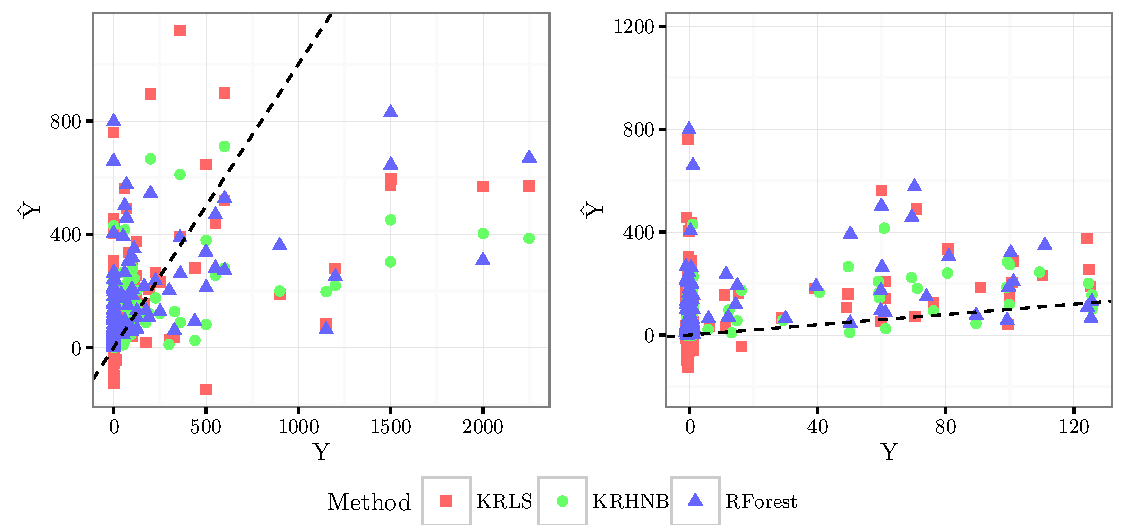
\includegraphics[width=0.95\linewidth]{tabs_figs/predictJoin.pdf}
	\caption{Leave-one-out CV Predictions}	\label{fig:predictions} 
	\begin{flushleft} \footnotesize \textit{Notes}: Black line is where perfect predictions would lie ($Y = \hat{Y}$). The left panel is the full dataset, while the right panel zooms in to where $Y < 150$. The values of $Y$ are jittered because of the clustering at 0. \end{flushleft}
\end{figure}

%=========================================================
\section{Results \& Discussion}	\label{sec:results} 	

\subsection{Data}

To uncover predictors of foreign fighter supply, we build a design matrix of $27$ geographic, demographic, economic, and political variables for $163$ countries. All of these features have been measured prior to 2014, although issues of endogeneity are beyond the scope of this paper. Furthermore, there is some (though very little) missingness, because we aggregate over several years (where applicable) to get as complete a dataset as possible. There is some remaining missingness, which we address by taking the mean over $1,000$ datasets, imputed using Amelia II \citep{Honaker2011}.\footnote{This algorithm relies on the assumption that the data are missing at random, which is almost certainly invalid. However, no feature has more than $4$ missing observations, save for the measure of how many refugees are in a country (missing $10$ observations). Furthermore, only 0.7\% of the data are missing.} In the Appendix Table~\ref{tab:appeffectslist}, we report full results with list-wise deletion, leaving us with $147$ observations. The results are largely the same.		\\

\begin{table}[!h]
	\footnotesize
	\centering
	\caption{Description of Features} 	\label{tab:data}
\begin{tabular}{lrrrrrl}
	\\ [-1.9ex] \toprule
	& Mean & Std. Dev. & Min. & Median & Max. & Source\\ 
	\midrule
	Foreign Fighter Supply & 114.08 & 332.34 & 0.00 & 0.00 & 2250.00 & ICSR \citep{Neumann2015}\\ 
	Contiguous & 0.04 & 0.20 & 0.00 & 0.00 & 1.00 & CEPII \\ 
	Europe & 0.21 & 0.41 & 0.00 & 0.00 & 1.00 & Hand Coded\\ 
	Distance (km) & 5251.69 & 3743.59 & 85.94 & 4363.00 & 15630.00 & CEPII \\ 
	Log Population & 16.23 & 1.51 & 13.20 & 16.15 & 21.03 & World Bank WDI \\ 
	Log Pop. Density & 4.19 & 1.40 & 0.60 & 4.30 & 8.95 & World Bank WDI\\ 
	Youth Bulge (15-24 pct) & 17.06 & 3.68 & 9.60 & 18.10 & 23.10 & World Bank WDI \\ 
	Sunni Pct & 25.45 & 35.33 & 0.07 & 5.07 & 99.40 & Pew \\ 
	Shia Pct & 2.61 & 10.82 & 0.00 & 0.06 & 92.22 & Pew \\ 
	Religious Frac. & 0.43 & 0.24 & 0.00 & 0.44 & 0.86 & \cite{Fearon2003a} \\ 
	Govt. Reg. Religion & 2.78 & 3.24 & 0.00 & 1.39 & 10.00 & ARDA \\ 
	Govt. Fav. Religion & 4.50 & 3.18 & 0.00 & 4.73 &  10.00 & ARDA \\ 
	Soc. Reg. Religion & 4.22 & 3.58 & 0.00 & 3.67 & 10.00 & Freedom House \\ 
	Freedom House Pol. Rights & 3.63 & 2.11 & 1.00 & 3.00 & 7.00 & Freedom House  \\ 
	Migrants as Pct of Pop & 7.87 & 12.06 & 0.05 & 2.94 & 74.61 & World Bank WDI\\ 
	Log Refugees in Country & 8.50 & 3.04 & 0.00 & 8.85 & 14.30 & UNHCR \\ 
	Log Refugees from Country & 7.35 & 2.92 & 0.00 & 7.18 & 14.75 & World Bank WDI \\ 
	Log GDP pc, PPP & 9.10 & 1.24 & 6.37 & 9.26 & 11.76 & World Bank WDI \\ 
	Life Expectancy & 69.89 & 9.48 & 45.55 & 72.27 & 83.83 & World Bank WDI\\ 
	Male LFP & 79.42 & 7.03 & 48.40 & 79.80 & 95.90 & World Bank WDI \\ 
	Youth Unemployment & 18.33 & 12.58 & 0.70 & 14.80 & 60.40 & World Bank WDI \\ 
	Internet User per 100 & 40.01 & 29.46 & 0.00 & 39.20 & 95.05 & World Bank WDI \\ 
	Log Homicides Per 100k & 1.46 & 1.20 & -1.61 & 1.57 & 4.50 & World Bank WDI \\ 
	\bottomrule
\end{tabular}
\begin{flushleft} \footnotesize \textit{Notes:} CEPII is the Centre d'\'{E}tudes Prospectives et d'Informations Internationales \citep{Mayer2011}. ARDA is the Association of Religion Data Archives \citep{Finke2010}. The Pew data can be found at in a report by \cite{Grim2012}. The Freedom House data are from \cite{Teorell2013}. The UNHCR data can be found at \href{http://popstats.unhcr.org/en/time\_series}{http://popstats.unhcr.org/en/time\_series} and are different from the World Bank summary of refugees in asylum because we exclude internally displaced persons. \end{flushleft}
\end{table}


The full list of features can be found in Table~\ref{tab:data}. We have data for all $163$ countries\footnote{We exclude Macao and Puerto Rico as well. They had high rates of missingness due to many organizations not collecting data on these polities.} with populations above $500,000$ except for Syria and Iraq, where our outcome is not measured. Foreign fighter data come from the ICSR Report of 1/25/2015 \citep{Neumann2015}, which estimates the number of all foreign fighters through the end of 2014. The estimates are either a single value, or a range. If there is a range, we take its mean, and round to the nearest integer.\footnote{ICSR also lack data from the West Bank and Gaza. In the interest of maximizing our sample size, we split the count for Israel and assign half of those sent from Israel to the West Bank and Gaza. Table~\ref{tab:appeffectslist} presents the results were we instead drop the West Bank and Gaza from our analysis, as well as other countries that have missingness. The results are substantively similar.} \\

\subsection{Main Results}

We fit KRHNB on the full data set, with $\lambda_{\psi}$ and $\lambda_{\omega}$ selected by a grid-search using leave-one-out cross validation. We use the Gaussian kernel to transform our data so that we are essentially working in an infinite-dimensional expansion of the design matrix and thus considering an infinite variety of complex functional forms. Following this optimization, we analyze the marginal effects of each feature on country-level foreign fighter supply in two ways. The first way is presented in Figure~\ref{fig:booteffects}, which contains the sample-average marginal effect and bootstrapped confidence intervals, for both the binary and count components, as well as the two components jointly. Note that the confidence intervals are constructed using the empirical 2.5th percentile and 97.5th percentile of the bootstrapped distribution of marginal effects.\footnote{This is sometimes known as the percentile interval, or the percentile bootstrap.} The exact results and confidence intervals for the sample-average marginal effects are presented in Table~\ref{tab:appeffects} of the Appendix. The bootstrapped intervals are skewed away from 0 for many sample-average marginal effects in the foreign fighters application, indicating that several outliers and the complex target function may prevent the bootstrapped percentile interval from achieving nominal coverage. \\

\afterpage{
\begin{landscape}
\begin{figure} [!p]
	\centering
	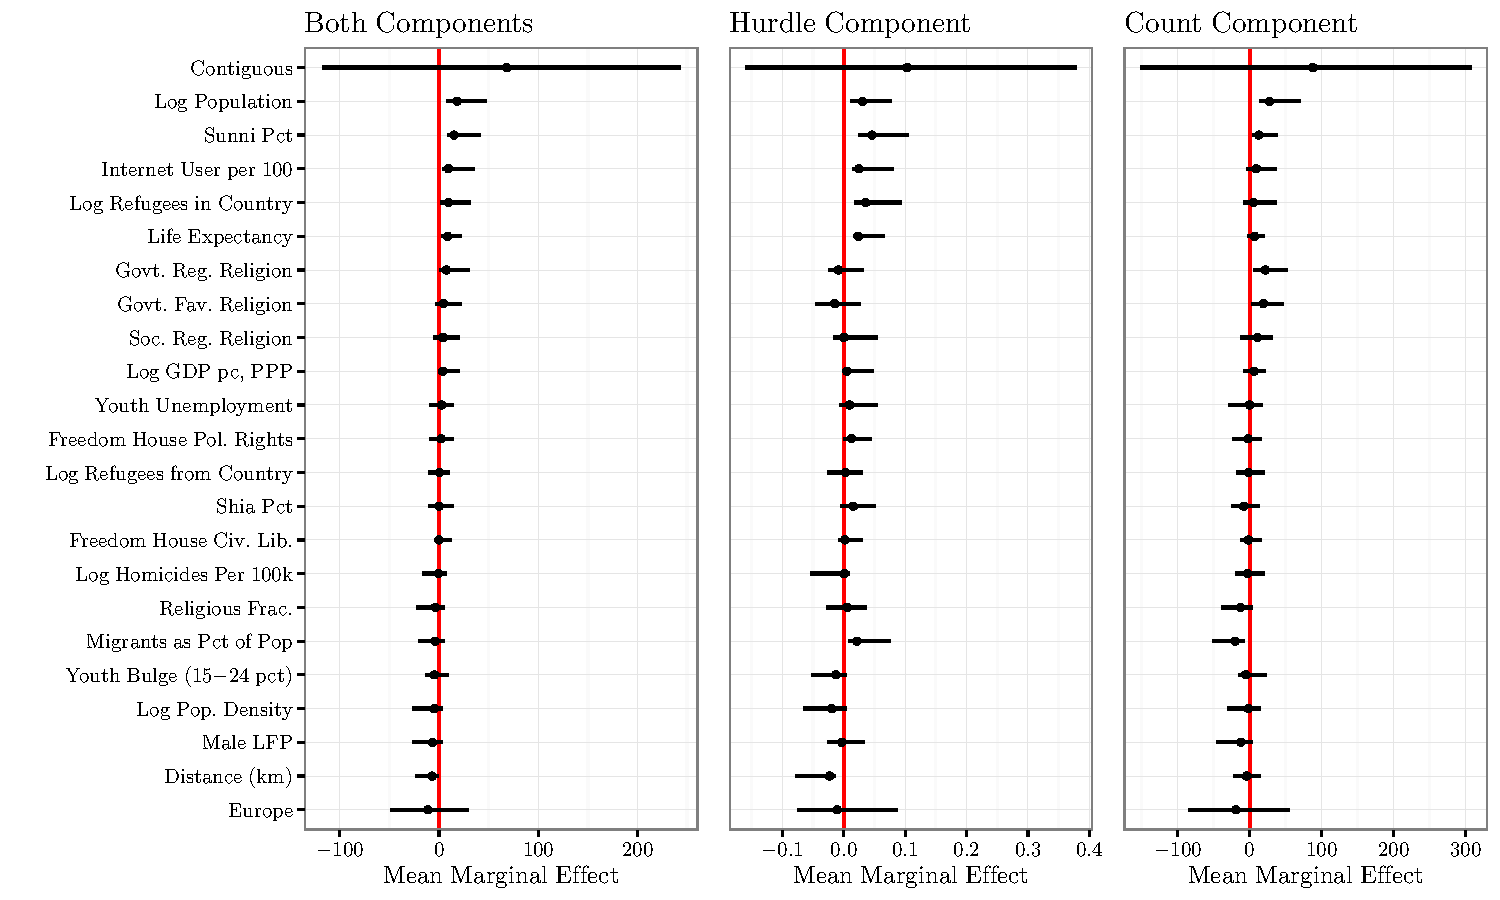
\includegraphics[scale=0.9]{tabs_figs/bootEffects.pdf}
	\caption{Sample-Average Pointwise Marginal Effects}		\label{fig:booteffects} 
	\begin{flushleft}
	\footnotesize \textit{Notes}: Pointwise marginal effects are computed numerically. All continuous features are scaled to have standard deviation of one. Dichotomous variables for Europe and Contiguous are not pointwise marginal effects, but first differences between the two values. Higher Freedom House scores indicate ``less freedom". The outcome variable is foreign fighter supply for the first column, the probability of sending any fighters in the hurdle logit component in the second column, and the mean of the truncated negative binomial component in the third column. As a result, note that the scaling of the $x$ axes varies. \end{flushleft}
\end{figure}
\end{landscape}
}

The leftmost panel of Figure~\ref{fig:booteffects} contains the estimated sample-average pointwise marginal effects for the combined model. Consistent with our usage throughout the paper, effects here mean the marginal effects our model produces, not causal effects. Furthermore, our features are scaled to have standard deviation of one so effects can be interpreted in standardized units. Most effects are near zero, showing that there is little predictive power for many of the features. Nonetheless, the bootstrapped 95 percentile intervals around seven of the features do not include 0. \\

Substantively, it appears that the two strongest predictors are population, and the percent of the country's population that is Sunni.\footnote{The point estimate for contiguity is quite large, although the low number of foreign fighters from Iran, a contiguous state to Iraq, is a source of the large heterogeneity in these marginal effects.} The effect of population is not surprising, as a positive (unconditional) probability of any individual becoming a foreign fighter implies that larger countries should have a higher supply. Similarly, Sunni population share intuitively predicts participation in the conflict, as it captures the strength of identification with the opposition; virtually all groups fighting the Assad regime are Sunni. Thus, more Sunnis in a given country means that more people feel they have a steak in the conflict and recruiters can more easily manipulate the salience of Sunnis' religious identity to construct a sense of obligation to fight. Also unsurprising is the strong negative effect of distance to the conflict; increased travel costs should deter potential fighters at the margin, while dissociation from the conflict should increase with distance. Another noteworthy effect is that on life expectancy, which positively predicts foreign fighter supply. Although this seems troubling, it is in line with popular conceptions of supplier countries as developed, as well as the findings of \cite{Hewitt2009} that more developed countries supplied more foreign fighters during Iraq's insurgency. Also consistent with conventional wisdom is the positive effect of internet usage; foreign fighters can be recruited online \citep{Hegghammer2011}, thus countries with deeper internet penetration allow recruiters to cast their net more widely. There also is a positive relationship between government regulation of religion and foreign fighter supply, something we discuss further below. Finally, a puzzling finding is the positive effect of refugee presence. Below we show that this effect originates in European countries, hence we defer its interpretation for now. 		 \\

More can be learned by disaggregating the effects into the hurdle and count components of our model. The central panel of Figure~\ref{fig:booteffects} contains the estimated sample-average pointwise marginal effects of standardized variables in the hurdle component. These effects can be interpreted as changes in the probability that a country passes the hurdle of no supply and sends some foreign fighters. The results are quite similar to the left panel, indicating that our features are better at predicting whether or not any foreign fighters are supplied (binary component), rather than how many are supplied (count component). Six of the seven predictors that are distinguishable from zero in the combined model remain so here, and their ranking in terms of substantive significance is also similar. Sunni population share, population, and refugee presence are still the three strongest predictors, again followed by internet penetration, distance to the conflict, and life expectancy. Government regulation of religion is not distinguishable from zero in this component. In addition, there are two new results worth noting. First, GDP per capita has a positive effect. This is consistent with the positive effect of life expectancy, popular conceptions regarding foreign fighters as originating in the developed world, and prior findings on Iraq \citep{Hewitt2009}. Second, migrant population share also has a positive effect. Yet, we hesitate to interpret this, as the effect is reversed in the count component. 	\\

The rightmost panel contains the estimated sample-average pointwise marginal effects of standardized variables in the count component. Only five features are clearly driving prediction of the count of foreign fighter supply. As in the combined model and hurdle component, population and Sunni population share have a positive effect distinguishable from zero. However, in contrast to the hurdle component, the effect of migrant population share is negative. Clearly, the opposite direction of the migrant effect in the two components accounts for its null effect in the combined model. Another difference from previous results is that government regulation of religion and government favoritism of religion are positive predictors.\footnote{These indices reflect how much the government respects freedom of religion, and whether it funds and supports one religion in particular \citep{Grim2006}.} This means that, among supplier countries, those that do not respect freedom of religion and/or fund a particular religion send more foreign fighters. Further inspection of these effects reveals that they are due to Sunni-majority countries, hence we interpret them later.	\\

\subsection{Effect Heterogeneity}

Our method allows for a rich exploration of marginal effect heterogeneity, by providing pointwise estimates of marginal effects for each feature. To demonstrate some of KRHNB's strength in learning from the data, Figure~\ref{fig:histeffects} plots the distribution of pointwise marginal effects for four features. Most of the effects are near zero, indicating that much of the estimated CEF is flat across the support of the features. However, a clear difference can be seen between a feature that appears to have little to no relationship to foreign fighter supply (homicides, bottom left), and one that has a systematic relationship (Sunni population share, bottom right). Heterogeneity in the pointwise marginal effects can itself provide a lot of information about certain features of interest. Furthermore, by plotting or regressing the pointwise marginal effects on the features, we can see whether there appear to be interaction effects, or non-linear relationships \citep{Hainmueller2013}. \\

\begin{figure}[!h]
	\centering
	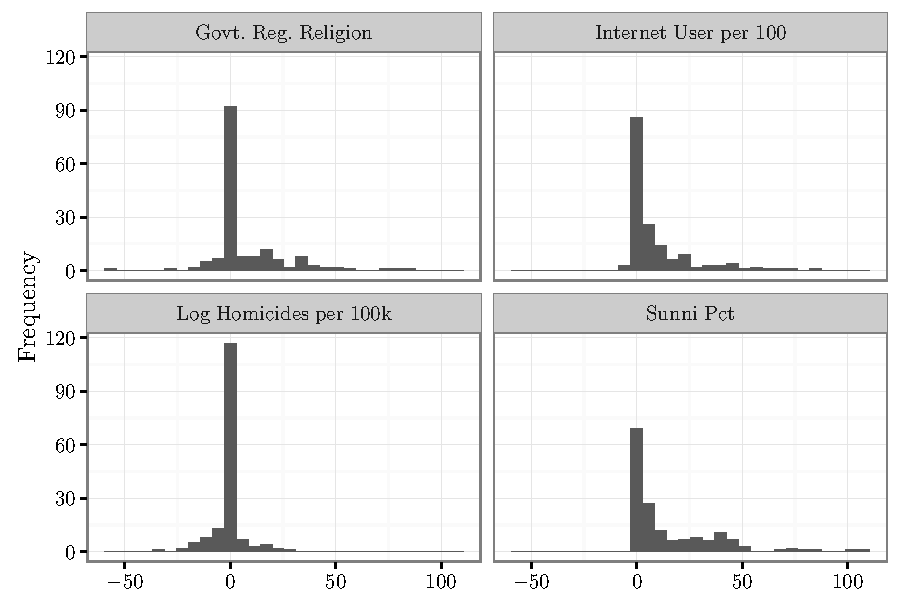
\includegraphics[scale=.85]{tabs_figs/histeffects.pdf}
	\caption{Distribution of Pointwise Marginal Effects}	\label{fig:histeffects} 
\end{figure}

In Figure~\ref{fig:hetplot1}, we demonstrate how the pointwise marginal effects differ for countries within and outside of Europe. While internet usage has uniformly positive effects in Europe, in the rest of the world its marginal effect is clustered around zero. This could suggest that radicalization and recruiting happens mostly online in European countries, but through non-digital means in other countries (e.g. personal networks, mosques). The plot can also shed light on the puzzling result on refugee presence, as it suggests that refugee presence is associated with larger foreign fighter supply only in Western countries. A possible interpretation is that refugees' predicament -- persecution, poverty, loss of family members -- exacerbates feelings of injustice among citizens of the host country that are already at high risk of becoming foreign fighters (e.g. young Sunni unemployed males in urban centers).\footnote{We believe it is unlikely that the positive effect of refugee presence means that refugees are more likely to fight in Syria, since there is no anecdotal evidence of refugees from Western countries becoming foreign fighters. We also note that our refugee measure predates the large influx of refugees from Syria into Europe; this rules-out the explanation that Syrians are seeking refuge in Europe, only to return to Syria as fighters.} The latter might view their participation in the Syrian conflict as a chance to address the conditions that resulted in refugees' predicament. Radicalization might be especially strong for citizens of the host country with a shared religion or ethnicity with the refugees, the more so if the refugees fled countries with similar conditions to those that sparked the Syrian conflict. This applies to refugees from a number of countries that repressed Islam(ists) -- for example, Algeria, Bosnia, Egypt, Iraq, Libya, Russia, and Tunisia  -- much like the Assad regime did in Syria.	 \\

\begin{figure}[!h]
	\centering
	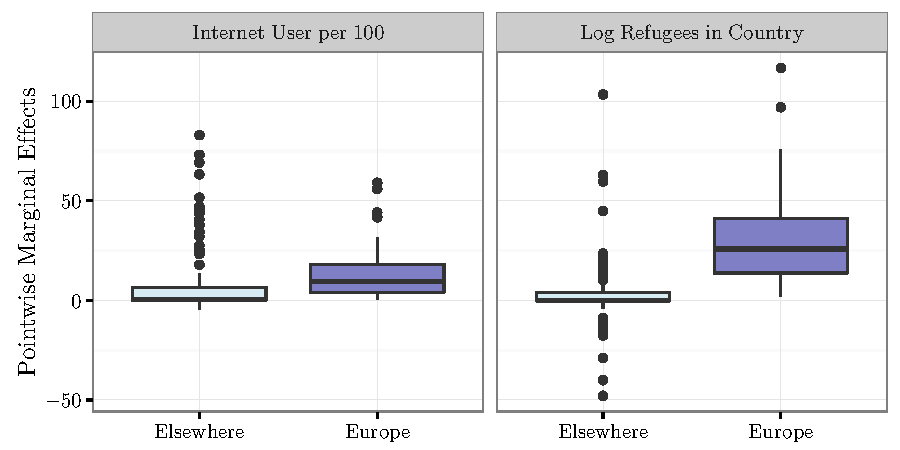
\includegraphics[scale=.85]{tabs_figs/hetplot1.pdf}
	\caption{Effects Inside and Outside Europe}	\label{fig:hetplot1} 
\end{figure}

This discussion provides an opportunity to return to the effect of government regulation of religion. As previewed above, intervention in religious affairs has a positive effect on foreign fighter supply in the model's count component. Figure~\ref{fig:hetplot2} reveals an interesting heterogeneity in this effect, by plotting the pointwise marginal effect of government regulation of religion by countries' Sunni population share with a simple LOWESS smoother.\footnote{To see the full picture of possible interaction effects, see Appendix~\ref{fig:interactplot} which presents an overview of heterogeneous effects.} As the Sunni share of the population increases the effect of government regulation of religion becomes stronger and more precise. That is, only in Sunni-majority supplier countries does religious intervention consistently predict a larger supply of foreign fighters. Given that virtually all foreign fighters are Sunni, this is consistent with a view of illiberal religious policies as radicalizing the population in Sunni-majority countries. This radicalization, in turn, might map onto foreign fighter supply through two possible mechanisms. One is that repressing (Sunni) Islam in countries where it is popular can create deep-seated grievances. Since the Assad regime also fought Islam, repressed Sunnis from the Muslim world might see Syria as a battleground for addressing their grievances. This could be the case in Tunisia, an overwhelmingly Sunni country that repressed Islamists until 2011, and has by far the largest per capita supply of foreign fighters. The second mechanism is that government repression of some religions or sects to benefit the official state religion might lead to exporting this attitude abroad. Thus, Sunnis from countries that enforce the dominance of Sunni Islam might consider it their duty to defend that religion wherever it is threatened, as in Syria. This could be the case of Saudi Arabia, which was founded on the radical Wahhabi (Sunni) interpretation of Islam, and has the second largest supply of foreign fighters.	\\

These possible explanations are raised by our model because it is able to uncover non-linear and interactive relationships without relying on the a priori specification of complex functional forms and without overfitting. Therefore, our model provides fodder for future work that should causally identify the mechanisms that may lead from government intervention in religion to the generation of foreign fighters.	 \\

\begin{figure}[!h]
	\centering
	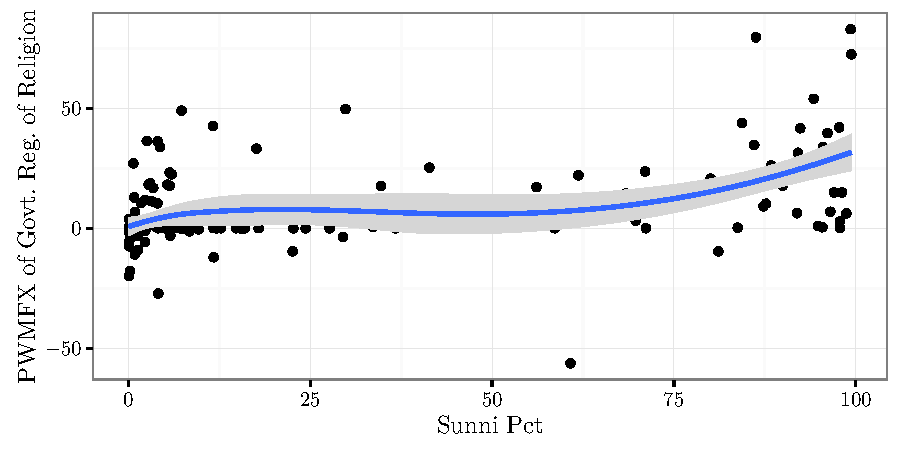
\includegraphics[scale=.85]{tabs_figs/hetplotGovtRegSunni.pdf}
	\caption{Effects of Government Regulation of Religion by Sunni Population Share}	\label{fig:hetplot2} 
\end{figure}

Overall, it seems that, while structural features dominate the hurdle component (distance, population, Sunni population share, life expectancy, GDP), policy variables mostly drive variation in the count component (government regulation of religion, government favoritism of a religion, migrant population share). Therefore, a tentative conclusion is that policy-makers cannot do much to prevent a foreign fighter network from emerging in their country, but, once it emerges, they can affect its size. Nevertheless, inspecting the effect of our features on the combined model, it is clear that structural features dominate in explaining foreign fighter supply, thereby limiting room for policy intervention.

%=========================================================
\section{Conclusion}	\label{sec:conclusion}

``The best way to reduce a foreign fighter returnee problem is to never have them go in the first place" \citep[p. 15]{Byman2015a}. Our analysis helps identify country features that are associated with higher foreign fighter supply. Substantively, our results suggest that countries' structural features play a larger role in shaping supply than their policies --- four of the strongest and most accurate predictors of supply are population, the share of the population that is Sunni, distance to Syria, and life expectancy. Some of these features cannot be altered by policy-makers, while others can, albeit at a slow pace and high cost. Moreover, with the exception of internet usage, all of the features that do respond to government policies -- refugee intake, regulation of religion, and favoritism of a particular religion -- are central to some countries' political culture. For example, French voters consistently prefer liberal policies towards refugees, while most Saudi citizens are likely to value state protection of Sunni Islam, and regulation of other religions. Therefore, policy-makers in such countries will hesitate to change these policies, unless the cost of doing so is less than that imposed by their foreign fighter supply. This might be unlikely, even for countries facing a high supply, like France and Saudi Arabia. In short, to the extent that our research design allows us to offer any policy recommendations, it is unclear whether policy-makers can feasibly curtail foreign fighter supply.	\\

Our approach is hindered by three limitations. On the empirical side, there is the inherent difficulty of measuring country-level foreign fighter supply. Fighters do not always publicize their participation in a conflict, not least because of fears of legal repercussions upon returning home. In addition, due to the nascent state of the literature, we lack a compass in our search for meaningful predictors to include in our specifications. Although we have carefully collected data on an array of economic, political, social, and demographic country features, there are many variables we have excluded from our specifications that may matter to foreign fighter supply. Future theoretical work will hopefully yield insights that can update our search for more informative predictors.		\\

Our second limitation is that our algorithm is computationally expensive. This is owed to three factors. First, our complex optimization problem (Equation \ref{eqn:targetFinal}) involves a large number of parameters (2$n$ + 3), and requires evaluating derivatives of the Gamma function. Second, our process for selecting the regularization parameters ($\lambda_\psi$, $\lambda_\omega$), involves a grid search and leave-one-out cross validation. Third, the difficulties of deriving an analytical estimate of uncertainty for our quantities of interest force us to resort to the bootstrap, which involves repeatedly refitting the model to resampled datasets. One of the authors is also working on lowering the dimensionality of a related problem to improve speed and provide estimates of uncertainty that avoid the bootstrap.	\\ 

On the theoretical side, a limitation of our framework is that it ignores psychological, ideological, and organization factors that figure prominently in the terrorism literature. This is inevitable, given that such factors are only observable at the individual- or group-level, while our analysis is at the country-level. In theory, one could collect data on confirmed fighters and match them to non-fighters, in an effort to identify individual-level predictors of their decision to go to Syria. Indeed, several recent papers based on interviews of a small sample of returning fighters focus on individual features, albeit through a purely descriptive qualitative approach \citep{Stenersen2011, Weggemans2014, Nilsson2015}. Expanding this dataset and applying classification models, such as Random Forest, is a promising avenue for future empirical research.	\\

In future work, we would like to generalize the model to allow for different parameterizations of the two components. For example, if we use the procedure to model individual choice, one may want to fit a probit to the binary component, motivated by a theory that the stochastic term is normally distributed. Similarly, if there is no over-dispersion in the truncated count, we may want to make efficiency gains by fitting a Poisson.\footnote{\cite{Zorn1998} notes that in the hurdle model over dispersion can be largely accounted for by the binary component, and thus a Poisson model may suffice for the count component.} Yet another extension is to allow for different features to enter each component. This is appropriate for questions where the theory guiding model specification is more developed. Nonetheless, with flexible estimators it is likely better to include as many relevant features as possible into the two components. 

Broader extensions of our method would involve applying it to different political science questions. KRHNB can be used to predict any count processes that might have a hurdle structure, ranging from the number of terrorist attacks perpetrated in each country (e.g. \cite{Burgoon2006}) to the number of bills passed by female legislatures in Congress (e.g. \cite{Volden2013}). Moreover, by abandoning the hurdle structure and applying kernel regularization to different classes of GLMs (e.g. binary choice), the range of political science processes that can be modeled becomes infinite. We hope that our study will motivate political methodologists to take up this task.	

%========================================================
\bibliography{ff}		\bibliographystyle{chicago}
%========================================================
\newpage
\appendix
\setcounter{table}{0}
\renewcommand{\thetable}{A\arabic{table}}
\setcounter{figure}{0}
\renewcommand{\thefigure}{A\arabic{figure}}
\setcounter{equation}{0}
\renewcommand{\theequation}{\Alph{section}.\arabic{equation}}
%========================================================
%========================================================
\section{Results Table and Heterogeneous Effects}	\label{app:tables}

\subsection{Full Results}

This section contains two tables that have the sample-average pointwise marginal effects for two different datasets. Table~\ref{tab:appeffects} contains the same information as Figure~\ref{fig:booteffects} and represents the results from our main specification where we impute missing values and divide foreign fighter supply between Israel and the West Bank. \\

\begin{table}[!p]
	\footnotesize
	\centering
	\caption{Average Marginal Effects on Foreign Fighter Supply} 	\label{tab:appeffects}
	\begin{tabular}{l ccc}
		\toprule
		Variable & \multicolumn{1}{c}{Both Components} & \multicolumn{1}{c}{Hurdle} & \multicolumn{1}{c}{Count} \\ 
		\midrule
Life Expectancy & 8.64 & 0.02 & 6.87 \\ 
& [2.88, 22.87] & [0.02, 0.07] & [-2.59, 21.3] \\ 
Contiguous & 68.3 & 0.1 & 87.89 \\ 
& [-117.95, 243] & [-0.16, 0.38] & [-151.81, 307.67] \\ 
Distance (km) & -6.99 & -0.02 & -4.36 \\ 
& [-23.87, -0.51] & [-0.08, -0.01] & [-21.98, 15.74] \\ 
Internet User per 100 & 9.48 & 0.02 & 9.37 \\ 
& [3.23, 36.21] & [0.01, 0.08] & [-4.11, 37.57] \\ 
Migrants as Pct of Pop & -3.84 & 0.02 & -20.19 \\ 
& [-20.76, 5.71] & [0.01, 0.08] & [-52.31, -7.87] \\ 
Male LFP & -6.52 & 0 & -12.23 \\ 
& [-26.61, 3.66] & [-0.03, 0.03] & [-46.65, 4.27] \\ 
Youth Unemployment & 2.73 & 0.01 & -0.12 \\ 
& [-9.21, 14.96] & [-0.01, 0.06] & [-29.94, 17.65] \\ 
Freedom House Civ. Lib. & -0.12 & 0 & -1.66 \\ 
& [-4.01, 12.74] & [-0.01, 0.03] & [-12.41, 15.97] \\ 
Freedom House Pol. Rights & 2.06 & 0.01 & -2 \\ 
& [-9.17, 15] & [0, 0.05] & [-23.41, 16.69] \\ 
Sunni Pct & 15.17 & 0.05 & 12.7 \\ 
& [8.06, 41.84] & [0.02, 0.11] & [3.92, 38.71] \\ 
Shia Pct & 0.19 & 0.02 & -8.48 \\ 
& [-11.1, 14.41] & [-0.01, 0.05] & [-25.07, 13.32] \\ 
Govt. Reg. Religion & 7.3 & -0.01 & 21.84 \\ 
& [0.34, 30.97] & [-0.02, 0.03] & [5.75, 52.54] \\ 
Govt. Fav. Religion & 4.45 & -0.01 & 19.11 \\ 
& [-3.94, 22.98] & [-0.05, 0.03] & [2.04, 46.65] \\ 
Soc. Reg. Religion & 3.96 & 0 & 10.8 \\ 
& [-5.36, 20.46] & [-0.02, 0.06] & [-12.12, 32.33] \\ 
Youth Bulge (15-24 pct) & -4.66 & -0.01 & -5.6 \\ 
& [-13.42, 9.51] & [-0.05, 0] & [-15.88, 23.18] \\ 
Religious Frac. & -3.8 & 0.01 & -12.71 \\ 
& [-22.42, 5.73] & [-0.03, 0.04] & [-38.91, 3.54] \\ 
Log Homicides Per 100k & -0.69 & 0 & -2.9 \\ 
& [-16.45, 7.97] & [-0.05, 0.01] & [-19.46, 20.01] \\ 
Log Pop. Density & -4.85 & -0.02 & -1.93 \\ 
& [-26.92, 3.47] & [-0.07, 0] & [-30.98, 15.26] \\ 
Log Population & 18.24 & 0.03 & 27.37 \\ 
& [7.31, 47.54] & [0.01, 0.08] & [13.14, 70.14] \\ 
Log GDP pc, PPP & 3.67 & 0.01 & 6.38 \\ 
& [-0.75, 20.31] & [0, 0.05] & [-7.99, 22.69] \\ 
Log Refugees in Country & 9.42 & 0.04 & 5.35 \\ 
& [1.4, 32.18] & [0.02, 0.09] & [-8.18, 36.92] \\ 
Log Refugees from Country & 0.55 & 0 & -1.34 \\ 
& [-10.9, 10.77] & [-0.03, 0.03] & [-18.47, 21.29] \\ 
Europe & -11.37 & -0.01 & -19.29 \\ 
& [-48.52, 29.19] & [-0.08, 0.09] & [-84.71, 55.31] \\ 
\midrule
N & 163 & & \\
		\bottomrule
	\end{tabular}
	\\ \footnotesize \textit{Notes}: The point estimates are the simple mean of pointwise marginal effects over the full data. The first column has the joint effect on the outcome of the full hurdle negative binomial model, while the second and third columns represent the effect on the probability of any fighters in the hurdle and the mean of the negative binomial distribution in the count component. In brackets are the 2.5th and 97.5th percentiles of the 1000 bootstrapped sample-average pointwise marginal effects. 
\end{table}

Table~\ref{tab:appeffectslist} contains the same results, but instead on a dataset where listwise deletion is used to remove observations with missing values. Furthermore, the West Bank and Gaza observation has been dropped rather than manually imputed. The results are very similar. The only substantive difference is that the percentile interval now includes 0 for the number of refugees in the country, although the effect is still strictly positive in the hurdle component.

\begin{table}[!p]
	\footnotesize
	\centering
	\caption{Average Marginal Effects on Foreign Fighter Supply in Listwise Deleted Dataset} 	\label{tab:appeffectslist}
	\begin{tabular}{l ccc}
		\toprule
		Variable & \multicolumn{1}{c}{Both Components} & \multicolumn{1}{c}{Hurdle} & \multicolumn{1}{c}{Count} \\ 
		\midrule
Life Expectancy & 15.24 & 0.04 & 12.01 \\ 
& [2.71, 35.62] & [0.01, 0.06] & [-9.94, 33.48] \\ 
Contiguous & 78.05 & 0.14 & 82.55 \\ 
& [-91.57, 266.88] & [-0.15, 0.34] & [-138.82, 304.3] \\ 
Distance (km) & -8.6 & -0.04 & 0.75 \\ 
& [-27.97, 4.96] & [-0.06, -0.01] & [-25.44, 35.02] \\ 
Internet User per 100 & 21.87 & 0.04 & 25.45 \\ 
& [4.38, 55.05] & [0.02, 0.07] & [-4.6, 65.7] \\ 
Migrants as Pct of Pop & -8.87 & 0.03 & -31.1 \\ 
& [-23.49, 8.55] & [0.01, 0.07] & [-67.27, -2.6] \\ 
Male LFP & -16.44 & 0 & -30.12 \\ 
& [-44.22, 0.94] & [-0.02, 0.03] & [-83.99, -1.16] \\ 
Youth Unemployment & 1.53 & 0.01 & -6.74 \\ 
& [-18.73, 18.49] & [-0.02, 0.05] & [-46.98, 25.33] \\ 
Freedom House Civ. Lib. & -2.27 & 0.01 & -8.71 \\ 
& [-7.19, 16.65] & [-0.01, 0.03] & [-20.98, 18.74] \\ 
Freedom House Pol. Rights & 0.65 & 0.03 & -11.18 \\ 
& [-17.51, 15.42] & [0, 0.04] & [-41.82, 15.94] \\ 
Sunni Pct & 26.57 & 0.07 & 23.85 \\ 
& [7.78, 52.81] & [0.03, 0.09] & [0.43, 54.28] \\ 
Shia Pct & -2.72 & 0.01 & -12.77 \\ 
& [-13.12, 15.71] & [-0.01, 0.04] & [-31.06, 19.03] \\ 
Govt. Reg. Religion & 14.75 & -0.01 & 34.68 \\ 
& [1.06, 43.85] & [-0.02, 0.03] & [3.94, 80.33] \\ 
Govt. Fav. Religion & 5.75 & -0.02 & 23.54 \\ 
& [-3.81, 31.51] & [-0.03, 0.03] & [-5.12, 67.13] \\ 
Soc. Reg. Religion & 8.3 & 0.01 & 13.15 \\ 
& [-4.82, 28.08] & [-0.01, 0.05] & [-13.39, 45.4] \\ 
Youth Bulge (15-24 pct) & -4.01 & -0.02 & -4.19 \\ 
& [-16.44, 15.04] & [-0.04, 0.01] & [-20.9, 34.81] \\ 
Religious Frac. & -6.56 & 0 & -16.27 \\ 
& [-32.4, 6.5] & [-0.03, 0.03] & [-58.49, 6.34] \\ 
Log Homicides Per 100k & 2.82 & 0 & 3.57 \\ 
& [-17.66, 16.3] & [-0.05, 0.01] & [-23.4, 40.09] \\ 
Log Pop. Density & -7.92 & -0.02 & -5.83 \\ 
& [-33.61, 6.05] & [-0.05, 0.01] & [-46.81, 20.93] \\ 
Log Population & 31.27 & 0.05 & 46.34 \\ 
& [7.58, 71.29] & [0, 0.06] & [14.38, 109.16] \\ 
Log GDP pc, PPP & 7.48 & 0.01 & 11.16 \\ 
& [-0.77, 30.97] & [0.01, 0.05] & [-11.26, 37.61] \\ 
Log Refugees in Country & 13.62 & 0.04 & 15.12 \\ 
& [-0.21, 47.45] & [0.01, 0.08] & [-9.63, 63.35] \\ 
Log Refugees from Country & -0.22 & -0.01 & 5.31 \\ 
& [-11.83, 19.31] & [-0.04, 0.01] & [-10.72, 47.96] \\ 
Europe & -11.1 & 0.01 & -25.47 \\ 
& [-71, 46.84] & [-0.08, 0.09] & [-135.44, 97.85] \\ 
\midrule
N & 147 & & \\
		\bottomrule
	\end{tabular}
	\\ \footnotesize \textit{Notes}: The point estimates are the simple mean of pointwise marginal effects over the full data. The first column has the joint effect on the outcome of the full hurdle negative binomial model, while the second and third columns represent the effect on the probability of any fighters in the hurdle and the mean of the negative binomial distribution in the count component. In brackets are the 2.5th and 97.5th percentiles of the 1000 bootstrapped sample-average pointwise marginal effects. 
\end{table}

\subsection{Heterogeneous Effects}

Because we able to compute pointwise marginal effects, it is possible to explore these effects to see how they vary in different parts of the feature space. One way to do this is simply to plot the pointwise marginal effects with respect to one variable by some other variable to see an interaction effect. A more robust way to explore these effects is to regress the pointwise marginal effects of some feature and all of the features in the data. This way, we can uncover the conditional interaction or non-linearity of our features. Of course, the pointwise marginal effects can themselves be modeled using flexible models or visualized using partial residual plots.  \\ 

A way to summarize all of these interaction effects is to regress the pointwise marginal effects for each feature on the full set of features. To be precise, we estimate a regression of the following form
$$ \frac{\partial\E[y_i|\x_i]}{\partial x^{(j)}_i} = \bm{\gamma}^\top \x_i,$$
where $x^{(j)}_i$ is the $i$th observation of the $j$th feature. We do this for all features $j$. The coefficients in $\bm{\gamma}$ are analogous to interaction terms ($\gamma_i \; \forall \; i \neq j$) or quadratic terms ($\gamma_j$). Thus if we are predicting the pointwise marginal effects of life expectancy on foreign fighter supply and we estimate a large positive $\gamma_i$ on, for example, the percent of the population that is Sunni, we then conclude that the marginal effect of life expectancy is much greater in heavily Sunni countries. Figure~\ref{fig:interactplot} contains the results of these regressions for all features, demonstrating how the variables interact. Large blue dots indicate the two have a positive interaction effect while large red dots indicate the two have a negative interaction effect.

\begin{figure}[!h]
	\centering
	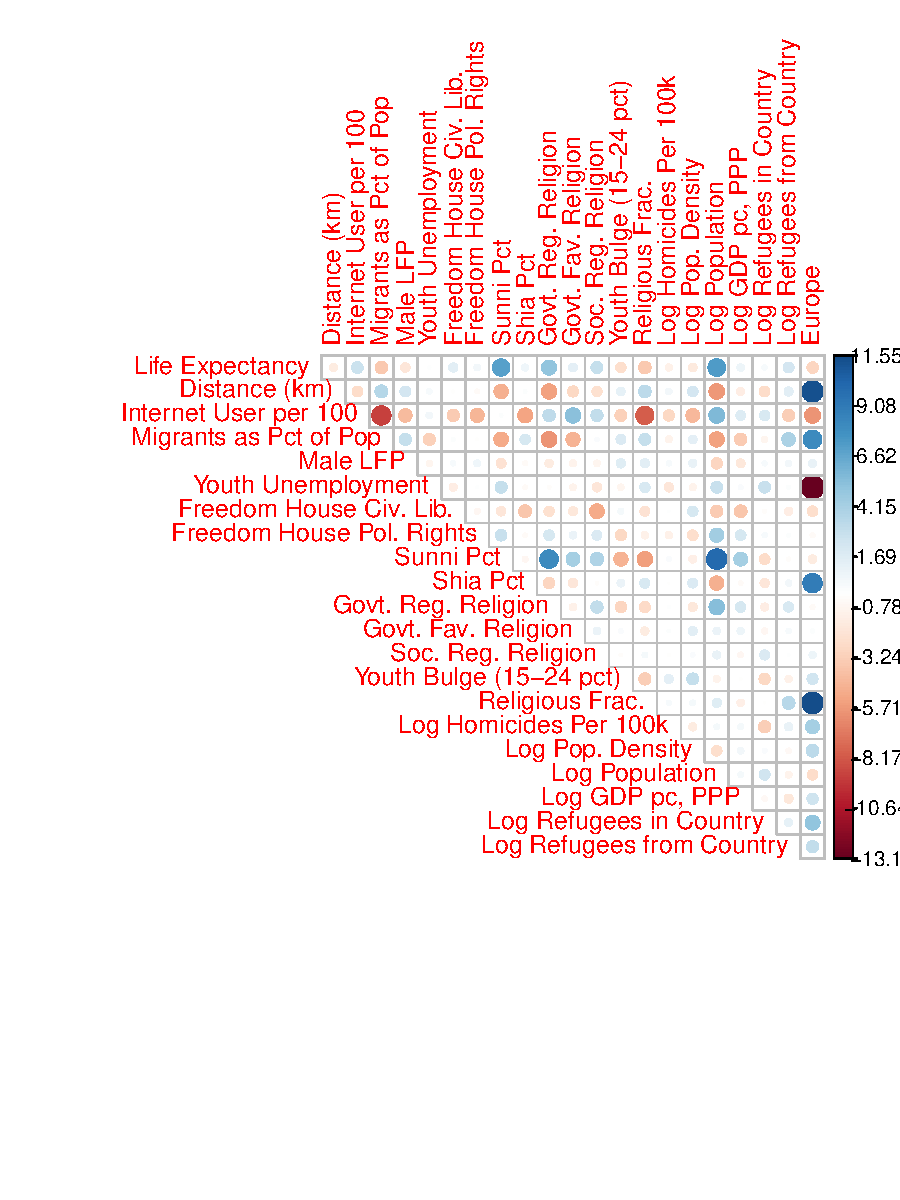
\includegraphics[scale=.85]{tabs_figs/interactPlot.pdf}
	\caption{Interaction Effects}	\label{fig:interactplot}
	\begin{flushleft} \footnotesize \textit{Notes}: Each cell is the coefficient from of a regression of one set of pointwise marginal effects on the rest of the data. A blue cell means that the two have a positive interaction while a red cell means the two have a negative interaction.	\end{flushleft}
\end{figure}

%========================================================
%========================================================
\section{Target Function Derivation}	\label{app:deriv}

\subsection{Sample Log-Likelihood}

The likelihood for observation $i$ in Equation~\ref{eq:likelihood} can be written more explicitly with respect to the densities in Equations~\ref{eq:dens0}, \ref{eq:densmu}, and \ref{eq:denstrunc}. Where $\btheta = (\alpha_0, \balpha^\top, \beta_0, \bbeta^\top, \zeta)^\top$,

\begin{align}
  L_i(\btheta | y_i, \x_i) &= \l[ p_0(y_i = 0) \r]^{1 - d_i} \l[ \frac{p_1(y_i)}{1 - p_1(y_ i = 0)} (1 - p_0(y_i = 0)) \r]^{d_i}
  \quad \text{;} \quad d_i = \begin{cases}
  0 \text{ if } y_i = 0 \\
  1 \text{ if } y_i \geq 1
  \end{cases}  \notag \\
  &= \l[ \frac{1}{1 + \exp(\alpha_0 + \x^\top_i \balpha)} \r]^{1 - d_i} \\
  &\times \l[ \frac{\Gamma (\zeta + y_i) \l( \frac{\zeta}{\zeta + \exp(\beta_0 + \x^\top_i \bbeta)} \r)^\zeta  \l( \frac{\exp(\beta_0 + \x^\top_i \bbeta)}{\zeta + \exp(\beta_0 + \x^\top_i \bbeta)} \r)^{y_i}}{\Gamma(1 + y_i) \Gamma(\zeta) \l( 1 -  \l( \frac{\zeta}{\zeta + \exp(\beta_0 + \x^\top_i \bbeta)} \r)^\zeta \r)} \frac{\exp(\alpha_0 + \x^\top_i \balpha)}{1 + \exp(\alpha_0 + \x^\top_i \balpha)} \r]^{d_i}
\end{align}

Next we derive the sample log-likelihood in Equation~\ref{eq:sampll}:

\begin{align}
\ell_N(\btheta | \Y, \X) &= \begin{aligned}[t]
\sum^N_{i=1} &(1 - d_i) \l[ \log 1 - \log \l( 1 + \exp(\alpha_0 + \x^\top_i \balpha) \r) \r] + d_i \Bigg[ \log \Gamma( \zeta + y_i ) \\
& + \zeta \log \zeta - \zeta \log \l( \zeta + \exp(\beta_0 + \x^\top_i \bbeta) \r) + y_i (\beta_0 + \x^\top_i \bbeta) \\
& - y_i \log \l( \zeta + \exp(\beta_0 + \x^\top_i \bbeta) \r) - \log \Gamma (1 + y_i) - \log \Gamma (\zeta) \\
&- \log \l(1 - \l( \frac{\zeta}{\zeta + \exp(\beta_0 + \x^\top_i \bbeta)} \r)^\zeta \r) + (\alpha_0 + \x^\top_i \balpha) \\
& - \log \l(1 + \exp(\alpha_0 + \x^\top_i \balpha) \r) \Bigg]
\end{aligned} \notag \\
 &= \begin{aligned}[t]
  \sum^N_{i=1} & - \log \l(1 + \exp(\alpha_0 + \x^\top_i \balpha) \r) +  d_i \Bigg[ \log \Gamma( \zeta + y_i ) + \zeta \log \zeta \\
  &- (\zeta + y_i) \log \l( \zeta + \exp(\beta_0 + \x^\top_i \bbeta) \r) + y_i(\beta_0 + \x^\top_i \bbeta) + (\alpha_0 + \x^\top_i \balpha) \\
  & - \log \Gamma (1 + y_i) - \log \Gamma (\zeta) - \log \l( 1 - \l( \frac{\zeta}{\zeta + \exp(\beta_0 + \x^\top_i \bbeta)} \r)^\zeta \r) \Bigg]
  \end{aligned}
\end{align} 

\subsection{Using Mercer's Theorem}

Given Equation~\ref{eqn:target}, we solve the First Order Condition (FOC) for each parameter vector in order to demonstrate our ability to use Mercer's Theorem to reduce our problem from a potentially infinite-dimensional one to a more tractable function. Where $\btheta_{\bphi} = (\psi_0, \bpsi^\top, \omega_0, \bomega^\top, \zeta)^\top$,

\begin{align}
\frac{\partial R_N (\btheta_{\bphi}, \lambda_\psi, \lambda_\omega | \Y, \X)}{\partial \bpsi} &= 0 \notag \\
0 &= -\sum^N_{i=1} \Bigg( - \frac{\bphi(\x_i)^\top \exp \l( \psi_0 + \bphi(\x_i)^\top \bpsi \r)}{1 + \exp \l( \psi_0 + \bphi(\x_i)^\top \bpsi \r)} + d_i \bphi(\x_i)^\top \Bigg) + 2 \lambda_\psi \bpsi \notag \\
\bpsi &= \sum^N_{i=1} \Bigg\{ \frac{1}{2 \lambda_\psi} \Bigg( - \frac{\exp \l( \psi_0 + \bphi(\x_i)^\top \bpsi \r)}{1 + \exp \l( \psi_0 + \bphi(\x_i)^\top \bpsi \r)} + d_i \Bigg) \Bigg\} \bphi(\x_i)
\end{align}

\begin{align}
\frac{\partial R_N (\btheta_{\bphi}, \lambda_\psi, \lambda_\omega | \Y, \X)}{\partial \bomega} &= 0 \notag \\
0 &= \begin{aligned}[t]
- & \sum^N_{i=1} d_i \Bigg[ - \frac{(\zeta + y_i) \bphi(\x_i)^\top \exp \l( \omega_0 + \bphi(\x_i)^\top \bomega \r)}{\zeta + \exp \l( \omega_0 + \bphi(\x_i)^\top \bomega \r)} + y_i \bphi(\x_i)^\top \notag \\
& - \frac{-\zeta \l( \frac{\zeta}{\zeta + \exp \l( \omega_0 + \bphi(\x_i)^\top \bomega \r)} \r)^{\zeta - 1} \l( \frac{- \zeta \bphi(\x_i)^\top \exp \l(\omega_0 + \bphi(\x_i)^\top \bomega \r)}{\l( \zeta + \exp \l( \omega_0 + \bphi(\x_i)^\top \bomega \r) \r)^2} \r)}{1 - \l( \frac{\zeta}{\zeta + \exp \l(\omega_0 + \bphi(\x_i)^\top \bomega \r)} \r)^\zeta} \Bigg] \Bigg) \\
&+ 2 \lambda_\omega \bomega 
\end{aligned} \\ \notag \\
\bomega &= \begin{aligned}[t]
\sum^N_{i=1} & \Bigg\{ \frac{1}{2 \lambda_\omega} d_i \Bigg[ - \frac{(\zeta + y_i) \exp \l( \omega_0 + \bphi(\x_i)^\top \bomega \r)}{\zeta + \exp \l( \omega_0 + \bphi(\x_i)^\top \bomega \r)} + y_i  \\
& - \frac{\zeta \l( \frac{\zeta}{\zeta + \exp \l( \omega_0 + \bphi(\x_i)^\top \bomega \r)} \r)^{\zeta - 1} \l( \frac{\zeta \exp \l(\omega_0 + \bphi(\x_i)^\top \bomega \r)}{\l( \zeta + \exp \l( \omega_0 + \bphi(\x_i)^\top \bomega \r) \r)^2} \r)}{1 - \l( \frac{\zeta}{\zeta + \exp \l(\omega_0 + \bphi(\x_i)^\top \bomega \r)} \r)^\zeta} \Bigg] \Bigg\}  \bphi(\x_i)
\end{aligned}
\end{align} 

Note that in both FOCs, the terms inside $\{\}$ form a scalar, which we label $c^\psi_i$ and $c^\omega_i$. As such, we rewrite our solutions for $\bpsi$ and $\bomega$ like we did in the main body of the paper:

\begin{align}
\bpsi^* = \sum^N_{i=1} c^\psi_i \bphi(\x_i) \\
\bomega^* = \sum^N_{i=1} c^\omega_i \bphi(\x_i) 
\end{align} 

We use these solutions to rewrite Equation~\ref{eqn:target} as Equation~\ref{eqn:targetFinal}, our final target function.

\end{document}
%%% Local Variables:
%%% mode: latex
%%% TeX-master: t
%%% End: